\documentclass[english]{beamer}
\usepackage{mathptmx}
\usepackage[T1]{fontenc}
\usepackage[latin9]{inputenc}
\usepackage{url}
\usepackage{amsmath}
\usepackage{amssymb}
\usepackage{graphicx}
\usepackage{mathtools}
\usepackage{dsfont}
\usepackage{hyperref}

\makeatletter
\newcommand\makebeamertitle{\frame{\maketitle}}%
\AtBeginDocument{%
  \let\origtableofcontents=\tableofcontents
  \def\tableofcontents{\@ifnextchar[{\origtableofcontents}{\gobbletableofcontents}}
  \def\gobbletableofcontents#1{\origtableofcontents}
}
\setbeamertemplate{navigation symbols}{%
    \usebeamerfont{footline}%
    \usebeamercolor[fg]{footline}%
    \hspace{1em}
}

\definecolor{blue(pigment)}{rgb}{0.2, 0.2, 0.6}


\setbeamercolor{footline}{fg=black}
\setbeamerfont{footline}{series=\bfseries}
\setbeamercolor{frametitle}{fg=blue(pigment)}
\setlength{\leftmargini}{5pt}

\usepackage{lmodern}

\makeatother

\usepackage{babel}

 
\begin{document}

\title{\textcolor{blue(pigment)}{Text Analysis for Economics and Finance}}
\vspace{8pt} 
\author{Ruben Durante\\
\small{ICREA-UPF, BGSE, IPEG, CEPR}}
\date{\small{DIW, October 2020}}

\frame{\titlepage}
\setbeamercovered{dynamic}

%almost three-fourths of the wordsidentified as negative by the widely used Harvard Dictionary are words typically notconsidered negative in financial contexts.

%\begin{frame}{More on dictionary-based methods: sentiment analysis}
%\begin{itemize}
%\setlength{\itemsep}{0.8em}
%\item Sentiment analysis is a subfield of NLP that identifies and extracts opinions and sentiments from texts
%\pause
%\item Understanding emotions from text is challenging. Even humans can get misled, so do not expect a 100\% accuracy from computers
%\item A text may contain multiple sentiments at once. E.g., \\
%\vspace{2pt}
%\textcolor{blue}{\textit{``The intent behind the final season of Game of Thrones\\
%was great, but it could have been way better''}}
%\item How do we conclude whether the review is positive or negative?
%\item Also, computers cannot comprehend figurative speech, or understand the use of similes, metaphors, hyperboles, etc.
%\pause
%\item Two tools:
%\vspace{4pt}
%\begin{itemize}
%\setlength{\itemsep}{0.3em}
%\item Linguistic Inquiry and Word Count (LIWC)
%\item Valence Aware Dictionary and sEntiment Reasoner (VADER)
%\end{itemize}
%\end{itemize}
%\end{frame}

\begin{frame}{Sentiment analysis with short text: VADER}
\begin{itemize}
\setlength{\itemsep}{1em}
\item Valence Aware Dictionary and sEntiment Reasoner (VADER): lexicon-based sentiment analysis tool particularly suited for
social media content
\item A sentiment lexicon is a list of lexical features (e.g., words) labeled according to their semantic orientation as either positive, negative, or neutral
\item It has been quite successful dealing with social media texts, newspaper editorials, movie and product reviews.
\item It does not only classify text as positive, negative, or neutral, but also provides a composite score that combines all three
\item Does not require any training data; constructed from a generalizable human-curated sentiment lexicon. subcategory
\end{itemize}
\end{frame}

\begin{frame}{Hassan et al. (QJE, 2019): firm-level political risk}
\begin{itemize}
\setlength{\itemsep}{1.35em}
\item Another example of application of dictionary methods
\item But the construction and the use of the dictionary is innovative
\pause
\item \textcolor{blue}{Goal}: to construct a measure of political risk faced by individual US firms
\item \textcolor{blue}{Data}: 178,173 transcripts of quarterly earnings conference calls
\pause
\item \textcolor{blue}{Idea}: measure the share of the conversations between call participants and firm management centered around risks associated with political matters
\end{itemize}
\end{frame}

\begin{frame}{Hassan et al. (QJE, 2019): constructing the dictionary}
\begin{itemize}
\setlength{\itemsep}{0.9em}
\item Training library of political text archetypical of discussions of political topics, \textcolor{blue}{$\mathbf{P}$}
\item Training library of non-political text, archetypical of discussion of non-political topics, \textcolor{blue}{$\mathbf{N}$}
\pause
\item \textcolor{blue}{$\mathbf{P}$}: William T. Bianco and David T. Canon, \textit{American Politics Today}
\item \textcolor{blue}{$\mathbf{N}$}: Robert Libby, Patricia A. Libby, and Daniel G. Short's, \textit{Financial Accounting}
\pause
\item Each library is the set of all adjacent two-word combinations (``bigrams'') contained in the text
\item \textcolor{blue}{$\boldsymbol{P}\backslash \boldsymbol{N}:$} terms that are in the political texts but not in the non-political text
\end{itemize}
\end{frame}

\begin{frame}{Hassan et al. (QJE, 2019): constructing the dictionary}
\begin{itemize}
\setlength{\itemsep}{1.2em}
\item First key statistics for them is \textcolor{blue}{$f_{b,\boldsymbol{P}}/B_{\boldsymbol{P}}$}
\vspace{3pt}
\begin{itemize}
\setlength{\itemsep}{0.6em}
%\setlength{\itemindent}{-0.9em}
\item \textcolor{blue}{$f_{b,\boldsymbol{P}}$}: frequency of bigram \textcolor{blue}{$b$} in the political training library
\item \textcolor{blue}{$B_{\boldsymbol{P}}$} is the total number of bigrams in the political training library
\item \textbf{What is this?}
\item Relative term frequency of \textcolor{blue}{$b$ }in \textcolor{blue}{$P$}. Similar to \textcolor{blue}{$tf_{i,j}$}
\end{itemize}

\pause

\item Second key statistics is \textcolor{blue}{$\boldsymbol{1}\left[ b\in \boldsymbol{P} \backslash \boldsymbol{N}\right]$}
\vspace{3pt}
\begin{itemize}
\setlength{\itemsep}{0.6em}
%\setlength{\itemindent}{-0.9em}
\item Where \textcolor{blue}{$\boldsymbol{1}\left[ \cdot \right]$} is an indicator function.
\item This is an extreme way of doing an \textcolor{blue}{$idf_{b}$} across libraries. \textbf{Why?}
\item \textcolor{blue}{$idf_{b}$} would give more weight to terms that are ``special'' to library \textcolor{blue}{$\boldsymbol{P}$}, i.e. not as frequent in \textcolor{blue}{$\boldsymbol{N}$}.
\item Here the weight is set to 0 for all terms in \textcolor{blue}{$\boldsymbol{P}$} that are also in \textcolor{blue}{$\boldsymbol{N}$}.
\end{itemize}
\end{itemize}
\end{frame}

\begin{frame}{Hassan et al. (QJE, 2019): constructing the dictionary}
\vspace{-7pt}
\begin{center}
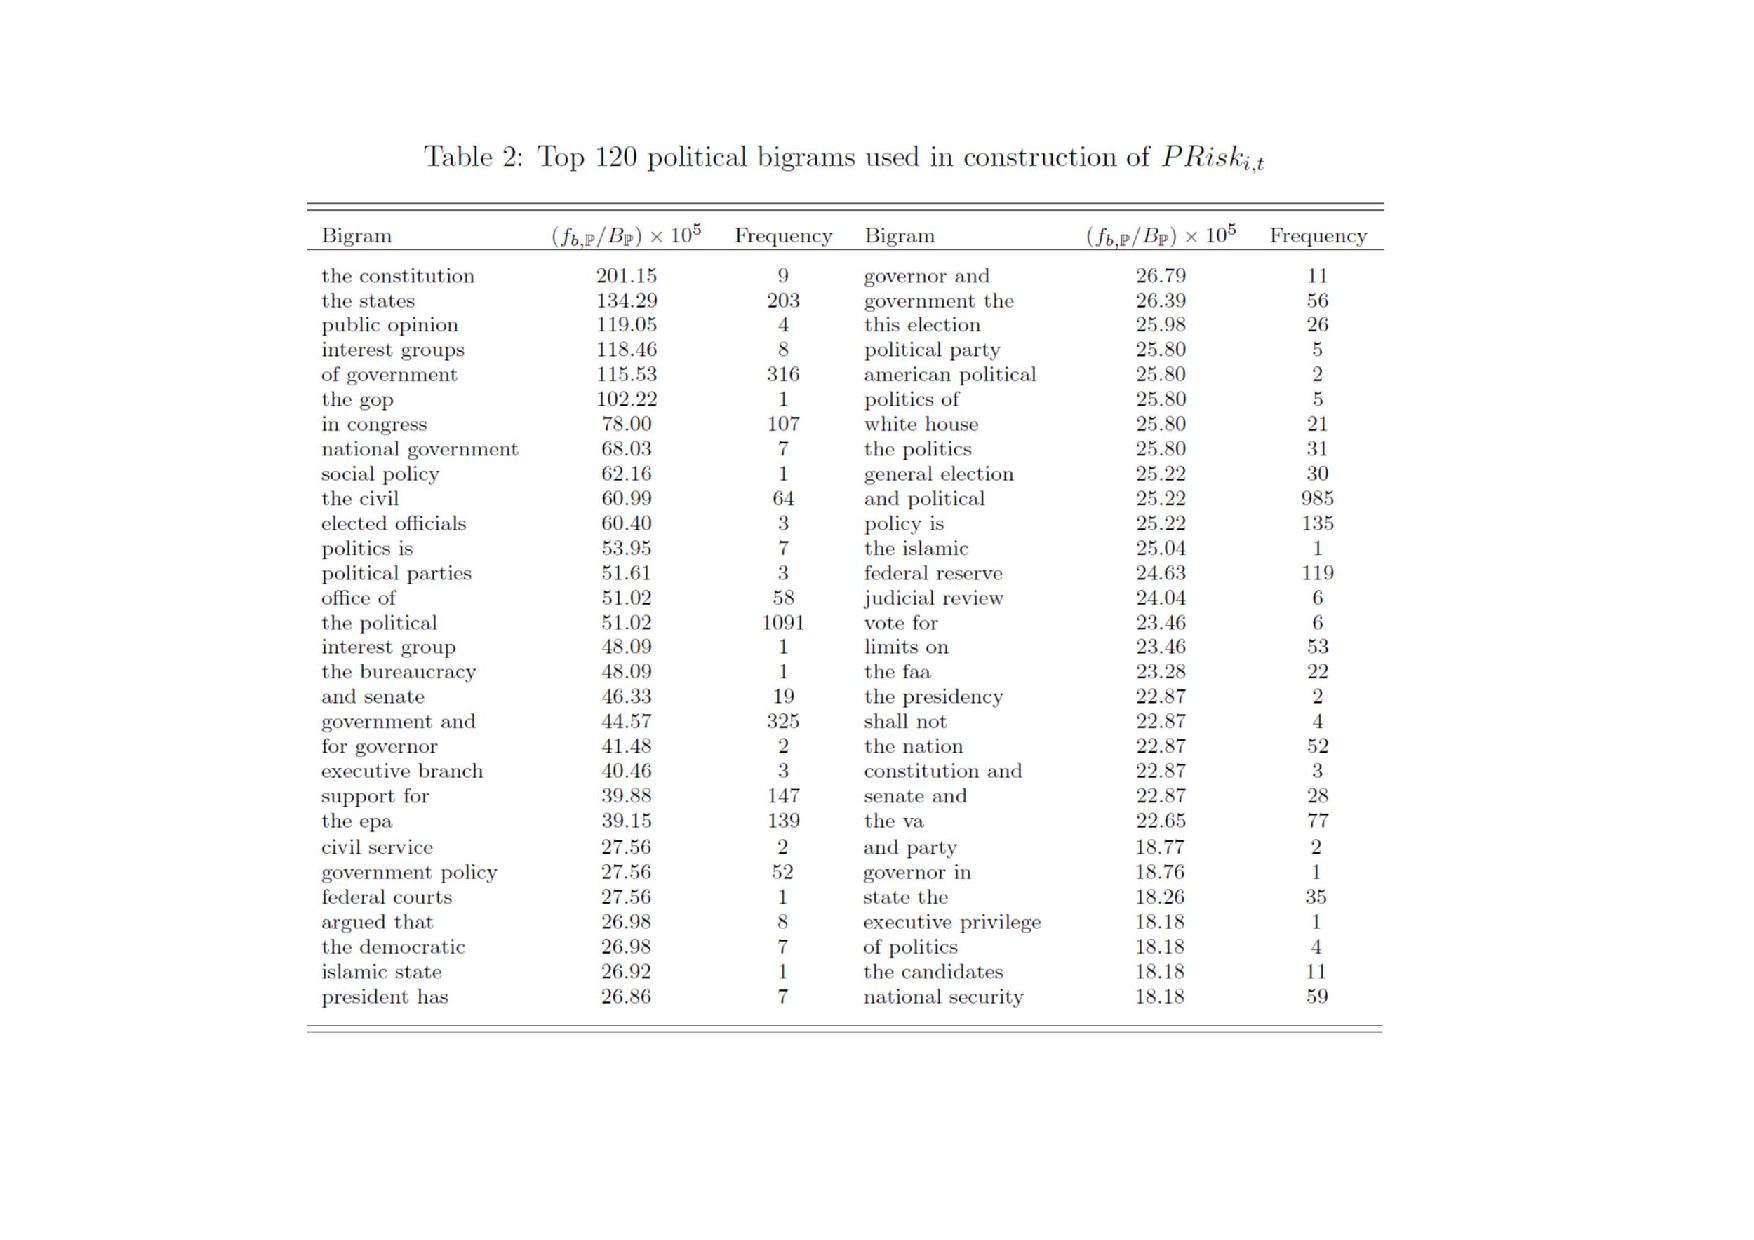
\includegraphics[scale=0.5]{Images/hassan_et_al_table1.pdf}
\end{center}
\end{frame}

\begin{frame}{Hassan et al. (QJE, 2019): using the dictionary}
\begin{itemize}
\setlength{\itemsep}{1.5em}
\item Count the number of instances where political bigrams are used in conjunction with synonyms for ``risk''
\item Conference-call transcript of firm $i$ in quarter $t$ into a list of bigrams contained in the transcript \textcolor{blue}{$b=1,...,B_{it}$}.
\vspace{7pt}
\textcolor{blue}{\begin{equation*}
PRisk_{it}=\frac{\sum_{b=1}^{B_{it}}\left( \boldsymbol{1}\left[ b\in 
\boldsymbol{P}\backslash \boldsymbol{N}\right] \times \boldsymbol{1}\left[
\left\vert b-r\right\vert <10\right] \times \frac{f_{b,\boldsymbol{P}}}{B_{%
\boldsymbol{P}}}\right) }{B_{it}}
\end{equation*}}
\item \textcolor{blue}{$r$} is the position of the nearest synonim for risk or uncertainty
\end{itemize}
\end{frame}%

\begin{frame}{Hassan et al. (QJE, 2019): using the dictionary}
\vspace{-7pt}
\begin{center}
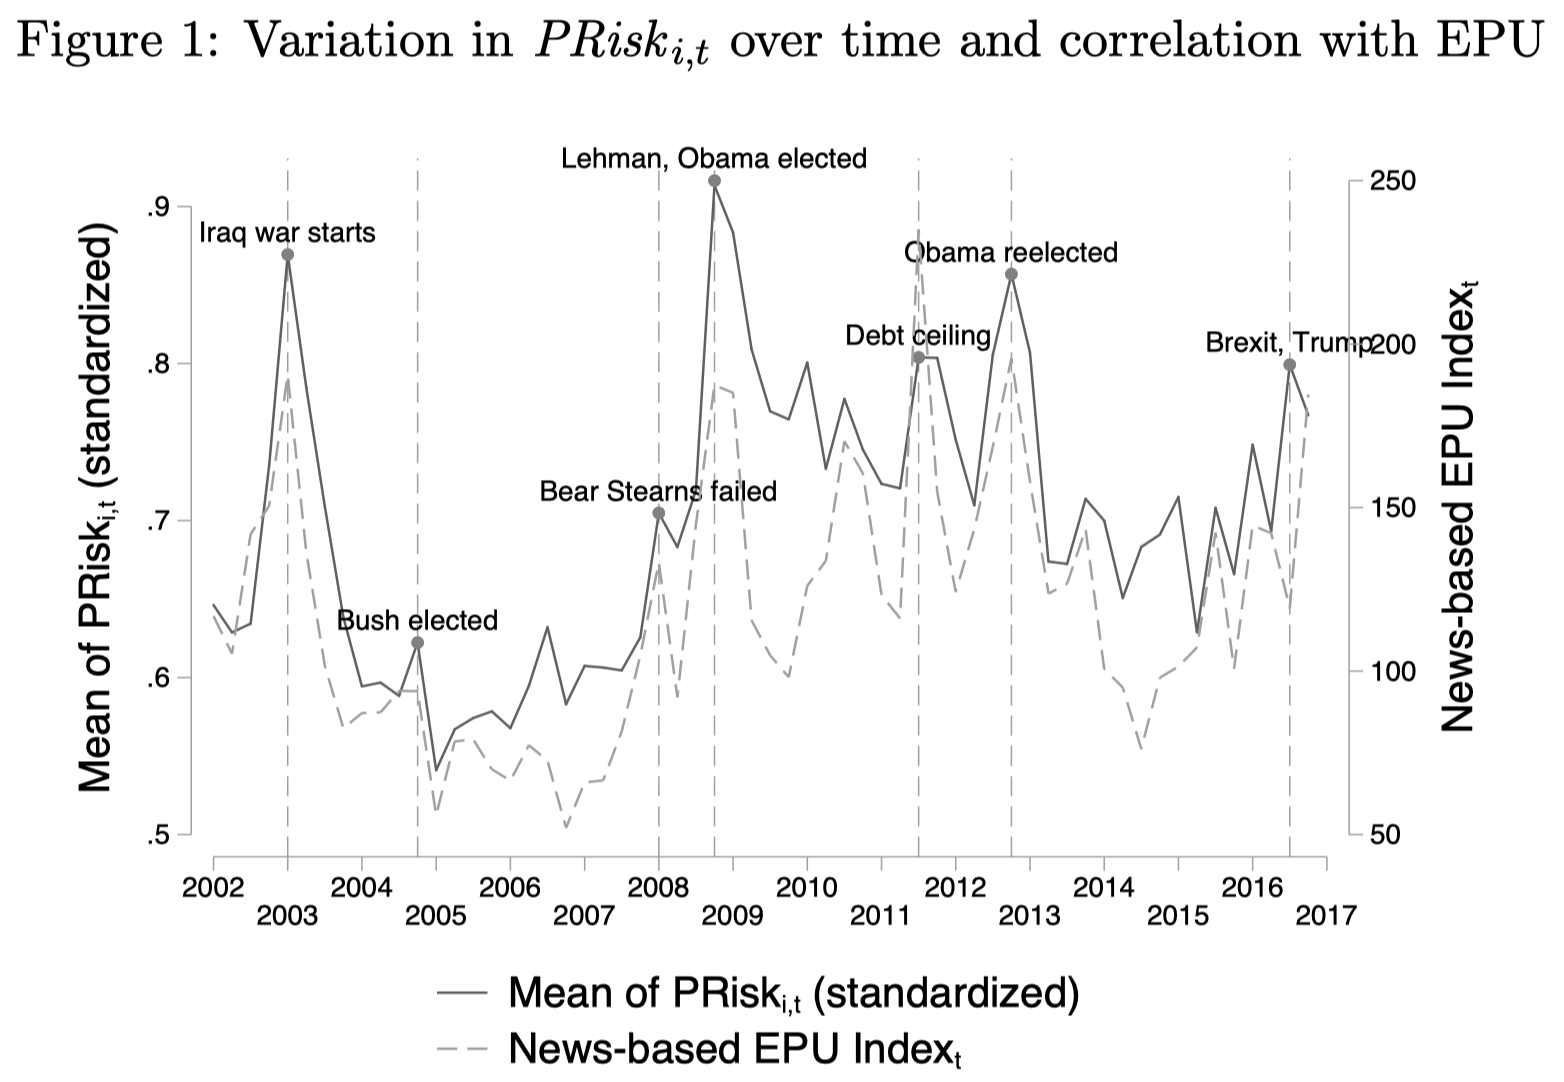
\includegraphics[scale=0.38]{Images/hassan_new1.png}
\end{center}
\end{frame}

\begin{frame}{Hassan et al. (QJE, 2019): using the dictionary}
\vspace{-7pt}
\begin{center}
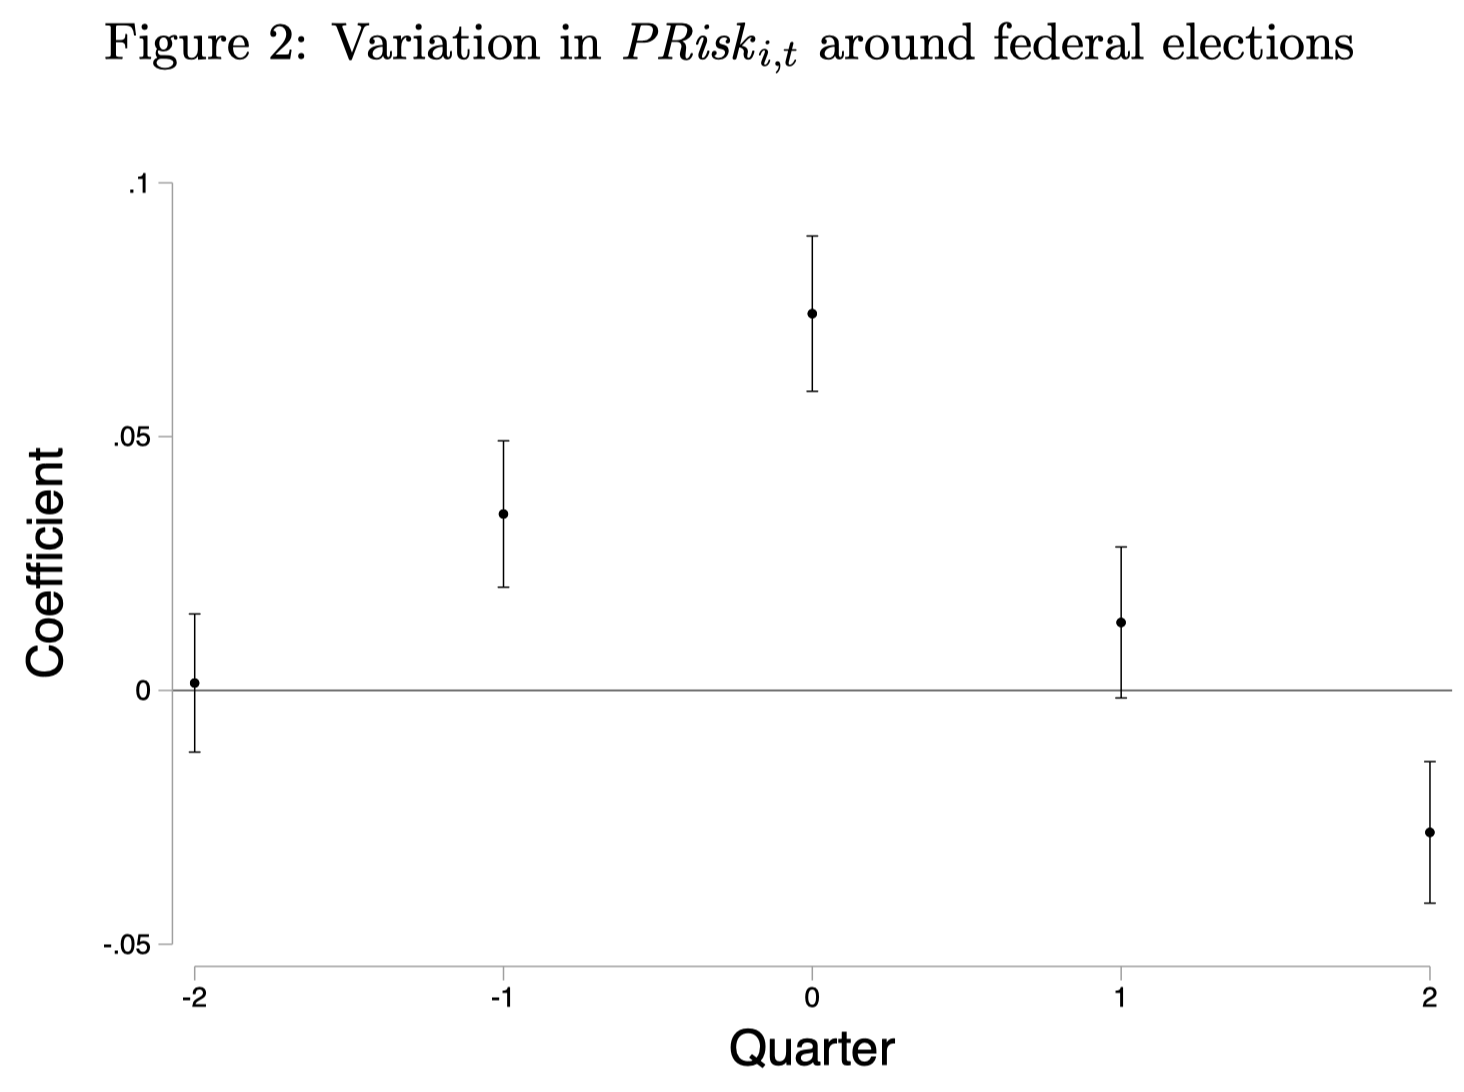
\includegraphics[scale=0.38]{Images/hassan_new2.png}
\end{center}
\end{frame}

\begin{frame}{Hassan et al. (QJE, 2019): using the dictionary}
\vspace{-7pt}
\begin{center}
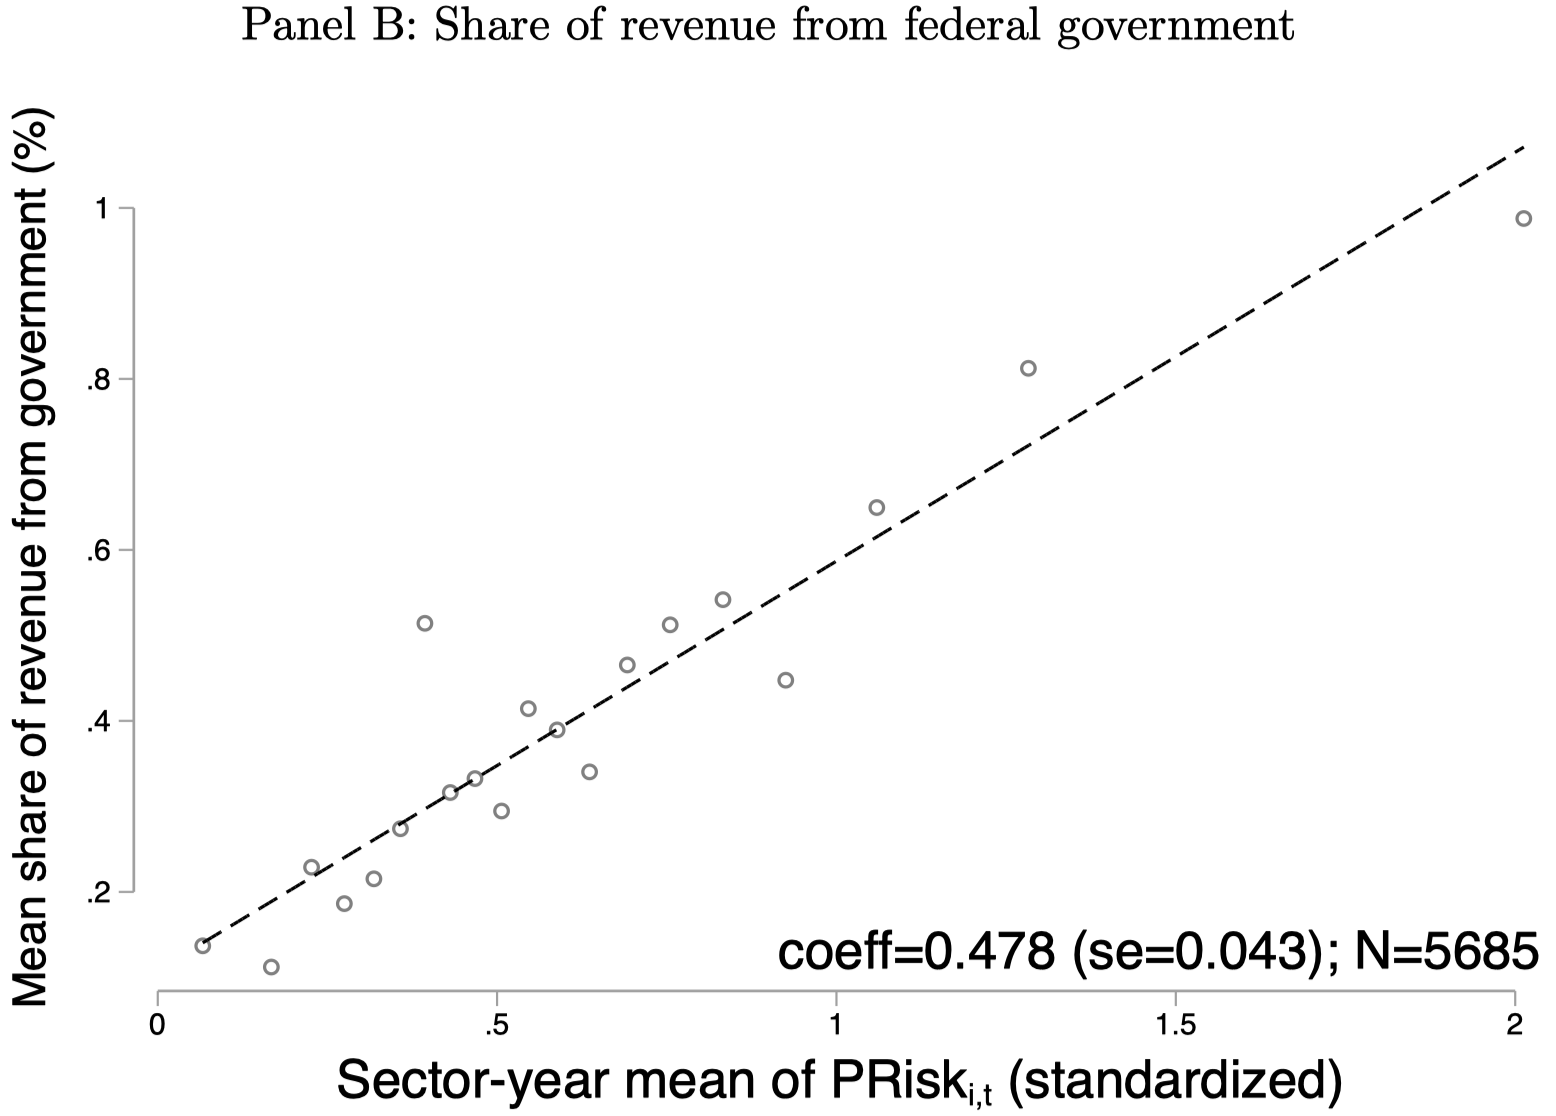
\includegraphics[scale=0.35]{Images/hassan_new3.png}
\end{center}
\end{frame}

\begin{frame}{Hassan et al. (QJE, 2019): using the dictionary}
\vspace{-7pt}
\begin{center}
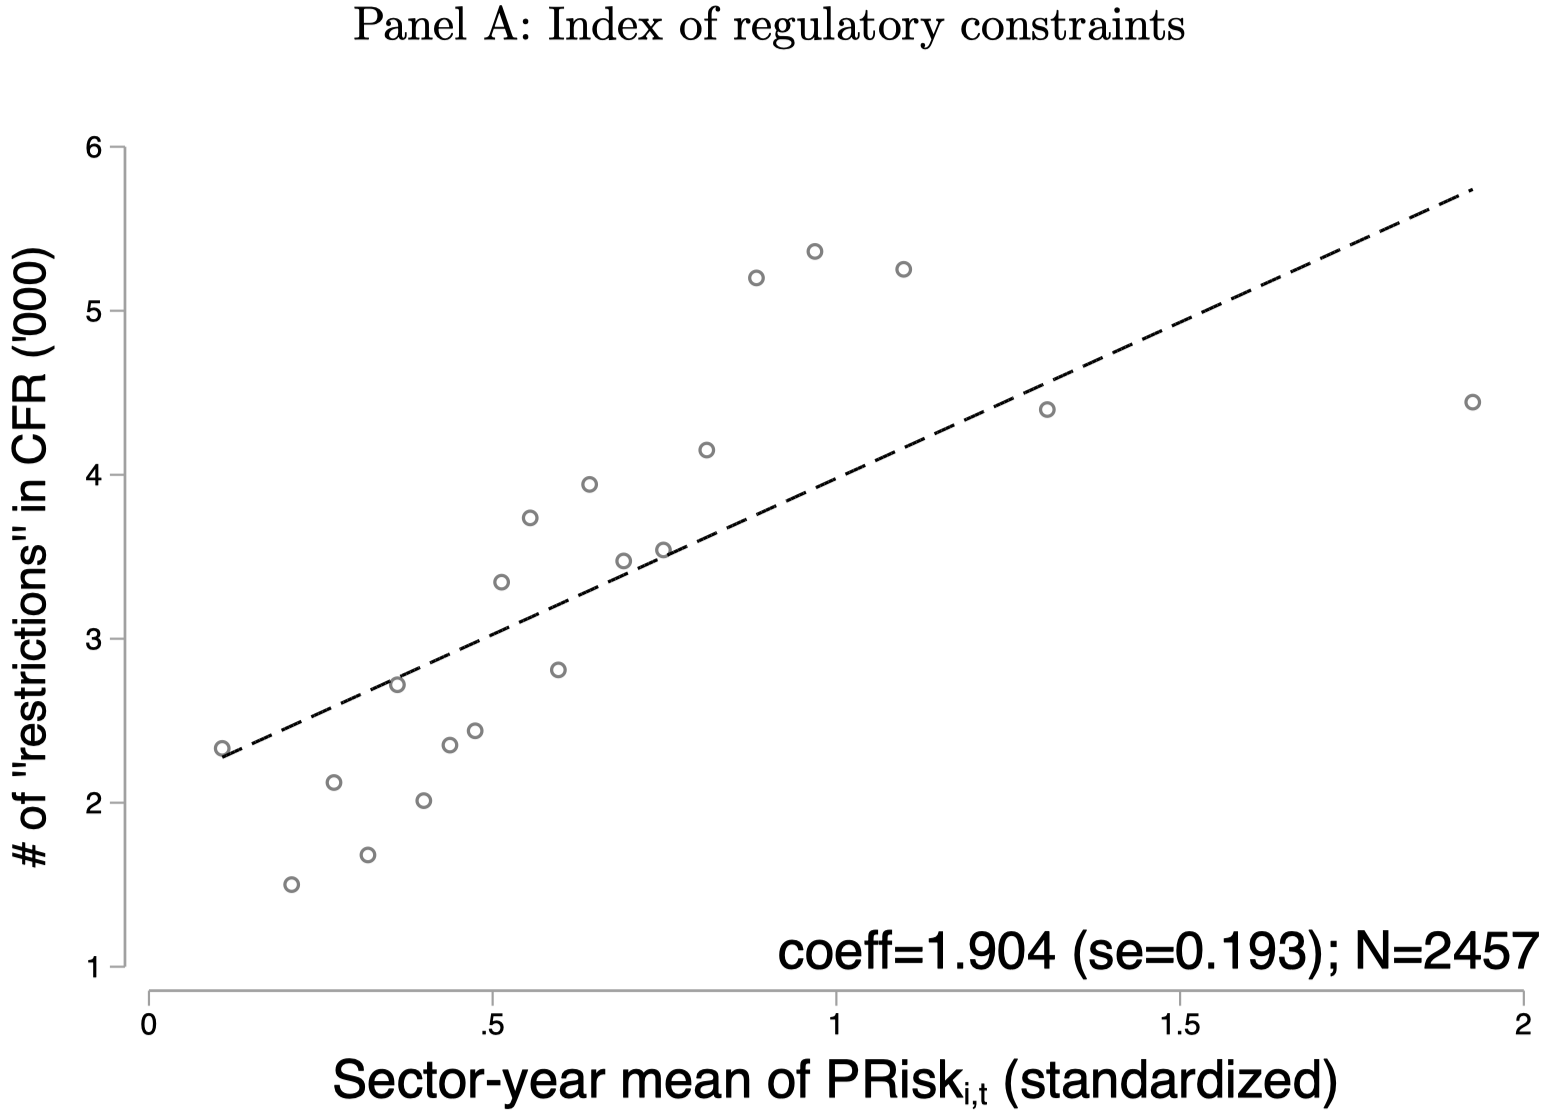
\includegraphics[scale=0.35]{Images/hassan_new4.png}
\end{center}
\end{frame}

\begin{frame}{Documents as vectors}
\begin{itemize}
\setlength{\itemsep}{1em}
\setlength{\itemindent}{-0.6em}
\item In the document-feature-matrix each document is represented by a\\
\hspace{-6.5pt}row-vector
\item Each vector contains the (weighted) frequencies of each feature in\\
\hspace{-6.5pt}the document
\item \textcolor{blue}{Idea}: these vectors can be used to measure the \textcolor{blue}{similarity/distance}\\
\hspace{-6.5pt}between documents
\end{itemize}
\end{frame}

\begin{frame}{Property of distance measures}
\begin{itemize}
\setlength{\itemsep}{1em}
\setlength{\itemindent}{-0.6em}
\item Let A and B be any two documents in a set and $d(A,B)$ be the\\
\hspace{-6.5pt}distance between A and B
\end{itemize}
\begin{enumerate}
\setlength{\itemindent}{-0.6em}
\setlength{\itemsep}{1em}
\item \textcolor{blue}{$d(x,y) \geq 0$}: the distance between any two points must be\\
\hspace{-6.5pt}non-negative
\item \textcolor{blue}{$d(A,B) = 0$ iff $A = B$}: the distance between two documents must\\
\hspace{-6.5pt}be zero if and only if the two objects are identical
\item \textcolor{blue}{$d(A,B) = d(B,A)$}: distance must be symmetric
\item \textcolor{blue}{$d(A,C) \leq d(A,B)+d(B,C)$} must satisfy the triangle inequality
\end{enumerate}
\end{frame}


\begin{frame}{Text analysis of patent innovation}

\framesubtitle{``Measuring technological innovation over the very long run'',
Kelly et al. (2019)}

\begin{itemize}
\setlength{\itemsep}{1em}

\item \textcolor{blue}{Goal}:
\vspace{5pt}
\begin{itemize}
\setlength{\itemsep}{0.4em}
\item Construct a new measure of \textcolor{blue}{novelty} and \textcolor{blue}{impact} of innovations based on similarity and distance between the text of patents

\pause{}

\end{itemize}


\item \textcolor{blue}{Data}:
\vspace{5pt}
\begin{itemize}
\setlength{\itemsep}{0.4em}
\item 9 million patents since 1840, from U.S. Patent Office and Google Scholar
Patents.
\item Date, inventor, backward citations
\item Text (abstract, claims, and description)

\pause{}

\end{itemize}

\item \textcolor{blue}{Text pre-processing}:
\vspace{5pt}
\begin{itemize}
\setlength{\itemsep}{0.5em}

\item Drop HTML markup, punctuation, numbers, capitalization, and stopwords
\item Remove terms that appear in less than 20 patents
\item 1.6 million words in vocabulary.
\end{itemize}
\end{itemize}
\end{frame}

\begin{frame}{Measuring Innovation}
\begin{itemize}
\setlength{\itemsep}{1em}

\item Backward IDF weighting of word \textcolor{blue}{$w$} in patent \textcolor{blue}{$p$}:
\textcolor{blue}{\[
\text{BIDF}(w,p)=\frac{\text{\# of patents prior to \ensuremath{p}}}{\text{log (1 + \# documents prior to \ensuremath{p} that include \ensuremath{w}) }}
\]}

\begin{itemize}
\item Down-weights words that appeared frequently before a patent, but up-weights
new words
\end{itemize}

\pause{}

\item For each patent:
\vspace{5pt}

\begin{itemize}
\item Compute cosine similarity to all future patents, using BIDF of earlier patent

\pause{}
\end{itemize}
\item 9m$\times$9m similarity matrix = 30TB of data
\vspace{5pt}
\begin{itemize}
\item Enforce sparsity by setting similarity < .05 to zero (93.4\% of pairs).
\end{itemize}
\end{itemize}
\end{frame}

\begin{frame}{Novelty, Impact, and Quality}
\begin{itemize}
\item ``Novelty'' is defined by (negative) similarity to previous patents:
\textcolor{blue}{\[
\text{Novelty}_{j}=-\sum_{i\in B(j)}\rho_{ij}
\]}
where \textcolor{blue}{$B(j)$} is the set of previous patents (in, e.g., last 20 years).

\pause{}

\vspace{5pt}

\item ``Impact'' is defined as similarity to subsequent patents:
\textcolor{blue}{\[
\text{Impact}_{i}=\sum_{i\in F(j)}\rho_{ij}
\]}
where \textcolor{blue}{$F(j)$} is the set of future patents (in, e.g., next 100 years).

\pause{}

\vspace{5pt}

\item A patent has high quality if it is novel and impactful:
\textcolor{blue}{\[
\text{Quality}_{i}=\frac{\text{Impact}_{i}}{-\text{Novelty}_{i}}
\]}
\end{itemize}
\end{frame}

\begin{frame}{Validation}
\begin{enumerate}
\setlength{\itemsep}{1.5em}
\item For pairs with higher \textcolor{blue}{$\rho_{i,j}$}, patent \textcolor{blue}{$j$} is more likely to
cite patent \textcolor{blue}{$i$}.

\item Patent office assigns 3-digit technology class code; similarity is
significantly higher within class compared to across class.
\item Higher quality patents get more cites:
\end{enumerate}
\end{frame}

\begin{frame}{Validation (cont.)}
\begin{center}
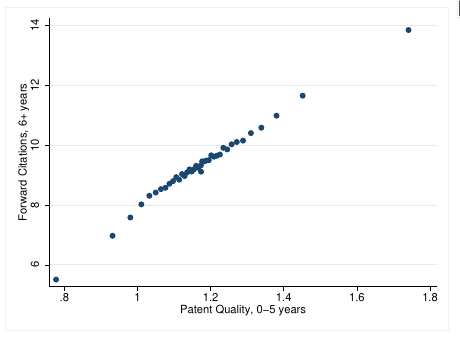
\includegraphics[width=0.5\textwidth]{Images/kelly-1}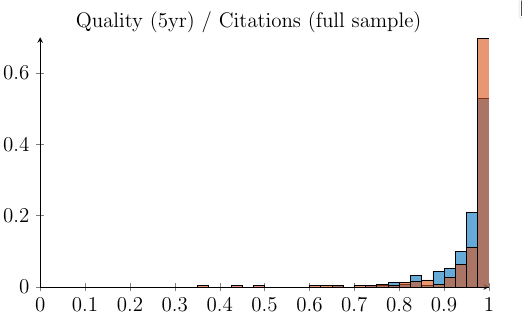
\includegraphics[width=0.5\textwidth]{Images/kelly-2}
\par\end{center}
\end{frame}

\begin{frame}{Most Innovative Firms}
\begin{center}
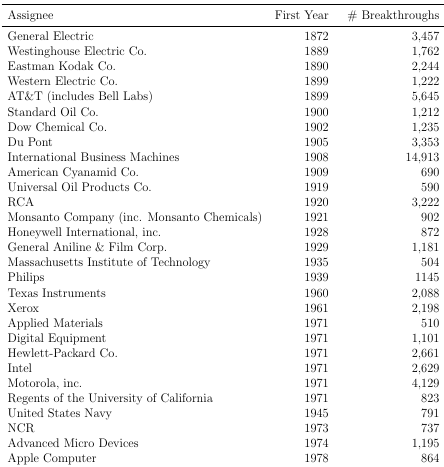
\includegraphics[height=0.8\textheight]{Images/kelly-7}
\par\end{center}

\end{frame}

%\begin{frame}{Patents per capita}
%\begin{center}
%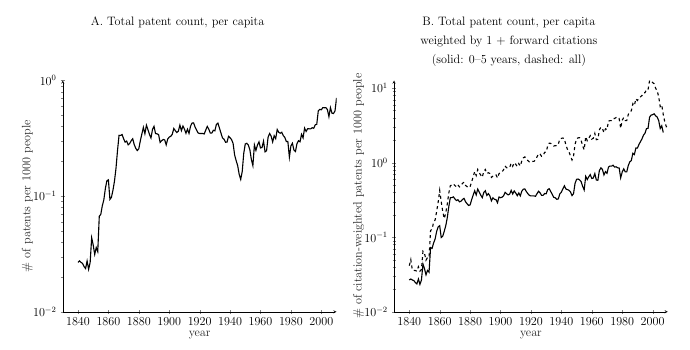
\includegraphics[width=1\textwidth]{kelly-3}
%\par\end{center}
%
%\end{frame}

\begin{frame}{Breakthrough patents per capita}
\begin{center}
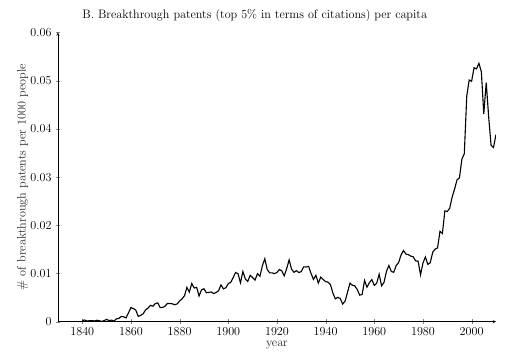
\includegraphics[width=0.5\textwidth]{Images/kelly-4}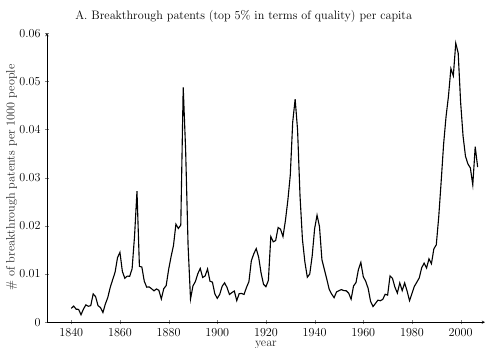
\includegraphics[width=0.5\textwidth]{Images/kelly-5}
\par\end{center}

\end{frame}

\begin{frame}{Breakthrough patents and firm profits}
\begin{center}
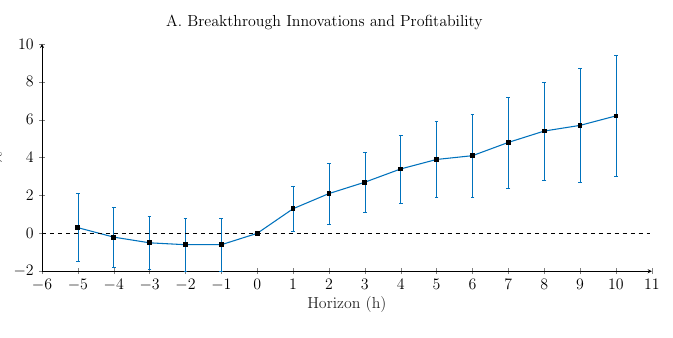
\includegraphics[width=1\textwidth]{Images/kelly-6}
\par\end{center}
\end{frame}

\begin{frame}{Jegadeesh and Wu (2013)}
\begin{itemize}
\setlength{\itemsep}{1.5em}
\item \textcolor{blue}{Goal}: estimate the response of a company's stock returns to information contained in the company's 10-K filings
\item \textcolor{blue}{Idea}: the content and wording of 10-Ks may prompt investor reactions in the following days which, in turn, can impact the firm's stock returns
\item Combine dictionary methods and text regressions to map the response of stock returns to the words included in a firm's 10-Ks
% First part of dictionary method is feature extraction (positive and negative words). The second part is how each word in the lexicon is weighted, which allows the algorithm to map descriptive content into a quantitative score. The existing weighting schemes (tf-idf) implicitly assumes that all words within a category are equally important (any positive word is equally impactful as a measure of positive)

% In this paper, the strength of various words as determinants of features is instead used as weights. That is, weights are assigned for each word based on market reactions (firm stock market returns) to documents (10-K fillings) containing those words

% The claim is that tf-idf is a somewhat crude and largely subjective way of weighting word relevances, and instead one can objectively extract word weight or relevance by regressing stock returns on these words. 
\item \textcolor{blue}{Main finding:} stronger and more stable relationship between the tone of 10-Ks and a firm's stock market returns than previously found using simpler word counting techniques
\end{itemize}
\end{frame}

\begin{frame}{Data}
\begin{itemize}
\setlength{\itemsep}{1.5em}
\item Use all 10-Ks filed from January 1995 through December 2010 from the SEC's \textcolor{blue}{EDGAR} database using a web crawling algorithm
\item The final sample contains 45,860 filings by 7,606 unique firms
\item For the dictionary, use the negative and positive word lists constructed by \textcolor{blue}{Loughran and McDonald (2011)} (LM).
\item The LM list contains \textbf{353} positive words and \textbf{2,337} negative words. By grouping similar words, the list is reduced to \textbf{123} positive words and \textbf{718} negative words
\end{itemize}
\end{frame}%
%
\begin{frame}{Empirical strategy}
\begin{itemize}
\setlength{\itemsep}{1.5em}
\item The objective is to fit the regression: 

\vspace{5pt}
\begin{center}
\textcolor{blue}{$
v_{i}=a+b\left(\sum_{j} w_{j} \frac{c_{i j}}{\sum_{j} c_{i j}}\right)+\varepsilon_{i}
$}
\end{center}
\vspace{5pt}
% The independent variable is their proposed word score, which contrasts the score that would be assigned by tf-idf and which should be correlated with the stock return that accompanies the release of document i. Said differently, they quantify the importance that the market attaches to each root word in the list at the time the information is revealed to the market.

% These regressions are at the document i level for a total of 45,860 regressions. Note that in their empirical application they measure v_i as excess returns by company vs. the CRSP value-weighted index. 

where \textcolor{blue}{$c_{ij}$} is a count of occurrences of word \textcolor{blue}{$j$} in 10-K report \textcolor{blue}{$i$}, \\
and \textcolor{blue}{$v_{i}$} is the company's stock excess returns in the post-filing days

\item The coefficient \textcolor{blue}{$w_j$} summarizes the average association between an occurrence of word \textcolor{blue}{$j$} and the stock's return
\item These coefficients are estimated using a cross-sectional regression, while a subsequent rescaling of all coefficients removes the common influence parameter \textcolor{blue}{$b$}.
\end{itemize}
\end{frame}%

\begin{frame}{Empirical Strategy (cont.)}
\begin{center}
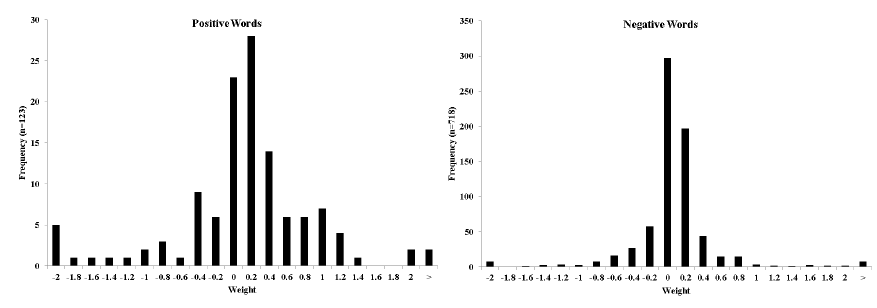
\includegraphics[scale=0.45]{Images/jegadeesh2013-1.png}
\vspace{7pt}
\begin{itemize}
\setlength{\itemsep}{0.5em}
\item The distribution of the resulting standardized LM word weights for positive and negative words
\item They emphasize that these weights are very different from those computed with simple tf-idf
% These are averages of the weights across all cross-sectional regressions, and for expositional purposes are demeaned and divided by the standard deviation across the respective cross sections. 
\end{itemize}
\end{center}
\end{frame}

\begin{frame}{Empirical Strategy (cont.)}
\vspace{-7pt}
\begin{center}
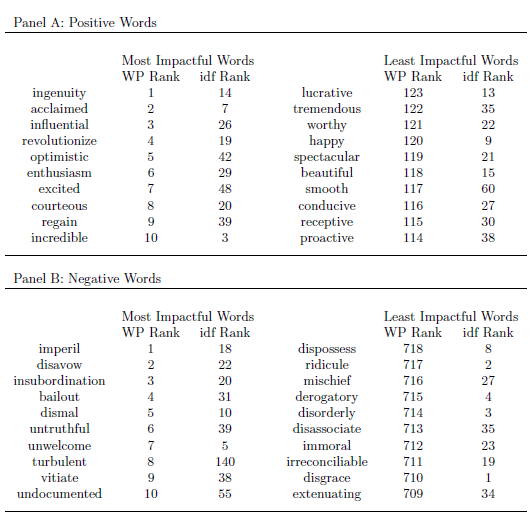
\includegraphics[scale=0.5]{Images/jegadeesh2013-2.png}
\begin{itemize}
    \item Weights rank substantially different from tf-idf counterparts 
% This highlights the contrast in weights assigned by the naive method (tf-idf) and the objective method (they call it word power weights)
\end{itemize}
\end{center}
\end{frame}

\begin{frame}{Results}
\vspace{-7pt}
\begin{center}
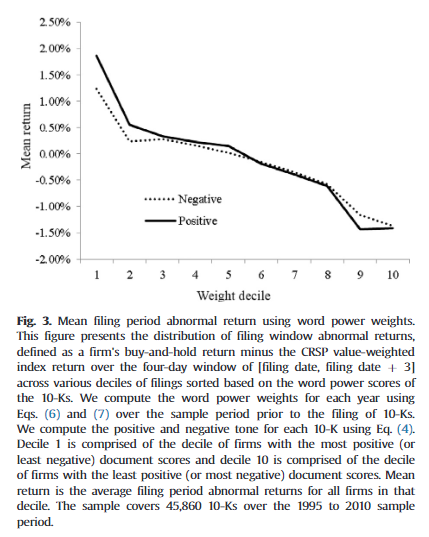
\includegraphics[scale=0.60]{Images/jegadeesh2013-3.png}
% This presents the average filing period returns for firms in various deciles of "positive talk" and "negative talk" (D1 consists of largest scores, D10 consists of lowest). Note that moving to the right represents a more negative tone (that is, more negative content or less positive content).
\end{center}
\end{frame}


\begin{frame}{Results (cont.)}
\begin{itemize}
\setlength{\itemsep}{1.5em}
\item Propose an approach to avoid subjectivity inherent to using lexicons composed of words with positive or negative connotations
% Further regressions of "filling period returns" on both word power and tf-idf scores show the former to yield stronger and more statistically significant results.

\item Move away from the idea that all positive or negative words ``count'' the same, let the data determine importance of each term for outcome

\item Robustness checks show that this weighting strategy reliably quantifies tone even when the subjectivity of the lexicon is increased
% The model's estimates are relatively stable even when limiting the LM lexicon. It is also robust to using the Harvard IV4 lexicon instead (the one Tetlock 2007 uses) 
\item Out-of-sample properties are superior to their dictionary-based counterparts. Highlight the limitations of the latter for purpose of prediction
\end{itemize}
\end{frame}


\begin{frame}{Manela and Moreira (2017): measuring NVIX}
\begin{itemize}
\setlength{\itemsep}{1.5em}
\item \textcolor{blue}{Goal}: construct an index of news-implied market volatility by identifying a small subset of words whose frequencies are most useful for predicting distress in financial markets

\item \textcolor{blue}{Idea}: relative coverage of topics by the business press is a good proxy for the evolution of investors' concerns about these topics
% They measure a news-based measure of uncertainty derived from the co-movement between WSJ front-page coverage and the VIX. This enables the construction of a VIX that spans far back in time and that can be interpreted (linked to words)
\item Use supervised machine learning (SVM) to identify relevant features from text and to build predictions of distress
% They rely on ML techniques to uncover information from WSJ data. They estimate the relationship between option prices and the frequency of words using support vector regression. This has the advantage over OLS in that it deals with a large feature space. 
\item \textcolor{blue}{Main finding:} news-implied volatility captures well the disaster concerns of the average investor over a long time span
% The NVIX predicts returns at frequencies from 6-to-24 months. This is consistent with asset pricing theory (NVIX measures fluctuation in expected stock market volatility). These results are robust to multiple specifications and in a word-decomposition (measured by regressing NVIX on individual n-grams and grouping similar categories) topics of war and government policy account for most of the variance in NVIX. 
\begin{itemize}
    \item War and government policy are good predictors of risk premia
\end{itemize}
\end{itemize}
\end{frame}%

\begin{frame}{Manela and Moreira (2017): data}
\begin{itemize}
\setlength{\itemsep}{1.3em}
\item Extract the title and abstract of all front-page articles of the Wall Street Journal from July 1889 to December 2009
\item Transform text data into \textcolor{blue}{$c_{it}$}, the relative frequency of over 400,000 n-grams
% n-gram counts are aggregated to a monthly frequency, and due to persistent changes in number of words x article and number of articles x day these are normalized by the total number of n-grams each month.

\item Volatility measured by the VIX implied volatility index
\item Break the sample into three subsamples:
\vspace{3pt}
\begin{itemize}
\setlength{\itemsep}{0.3em}
    \item \textcolor{blue}{\textit{Train} subsample} estimates the relation between news data and implied volatility using data from 1996 to 2009
% This is used to train how n-grams predict VIX
    \item \textcolor{blue}{\textit{Test} subsample} covers 1986-1995 and is used for out-of-sample tests of model fit
% This is used to check for out-of-sample performance and validate the calibration performed in the trained set
    \item \textcolor{blue}{\textit{Prediction} subsample} includes observations prior to 1986 for which features are not available
% With a well calibrated model, predict NVIX using WSJ from 1889 to 1985
\end{itemize}
\end{itemize}
\end{frame}%


\begin{frame}{Manela and Moreira (2017): empirical strategy}
\begin{itemize}
\setlength{\itemsep}{1.2em}
\item We need to estimate $$
VIX_{t}=w_{0}+\mathbf{w} \cdot \mathbf{x}_{t}+v_{t}
% n-grams are aggregated to a monthly frequency and normalized by total n-grams in the month, while n-grams with count<3 in the entire sample are omitted 
$$ but with OLS we will overfit ($T_{train} = 168$, $len(x_t) = 468,091$)
\pause
\item A solution is to use support vector regressions, which instead minimizes the following objective 
% SVR minimizes the l2 norm of the coefficient vector (instead of MSE). The error is handled as a constraint, with a tolerance margin defined as epsilon (Epsilon needs to be tuned). The model's performance is enhanced by slack variables, which allow for a flexible way to deviate from the epsilon margin. 

% This helps greatly reduce the dimensions the model uses to fit a line (since it instead fits it given tolerated errors. Thus, SVR selects a small number of observations (called Support Vectors) and ignores the rest, allowing only a handful of T_train observations being used for estimation.
$$
L\left(\mathbf{w}, w_{0}\right)=\sum_{t \in t r a i n} g_{\epsilon}\left(v_{t}-w_{0}-\mathbf{w} \cdot \mathbf{x}_{t}\right)+c(\mathbf{w} \cdot \mathbf{w})
$$
where $g_{\varepsilon}(e)=\max \{0,|e|-\varepsilon\}$ is an $\varepsilon$-insensitive error
% \item Hyperparameters are $\varepsilon$ and regularization parameter $c$
\pause
\item The minimizing coefficients vector \textcolor{blue}{$w$} is a weighted average of regressors $$
\hat{\mathbf{w}}_{S V R}=\sum_{t \in \text {train}}\left(\hat{\alpha}_{t}^{*}-\hat{\alpha}_{t}\right) \mathbf{x}_{t}
$$
% This restricted form does not consider each K linear subspace separately, which greatly reduces an overdetermined problem of finding K >>> T coefficients to a feasible linear-quadratic optimization problem with only a handful of parameters. 

\end{itemize}
\end{frame}%

\begin{frame}{\small{Manela and Moreira (2017): estimation results}}
\vspace{-7pt}
\begin{center}
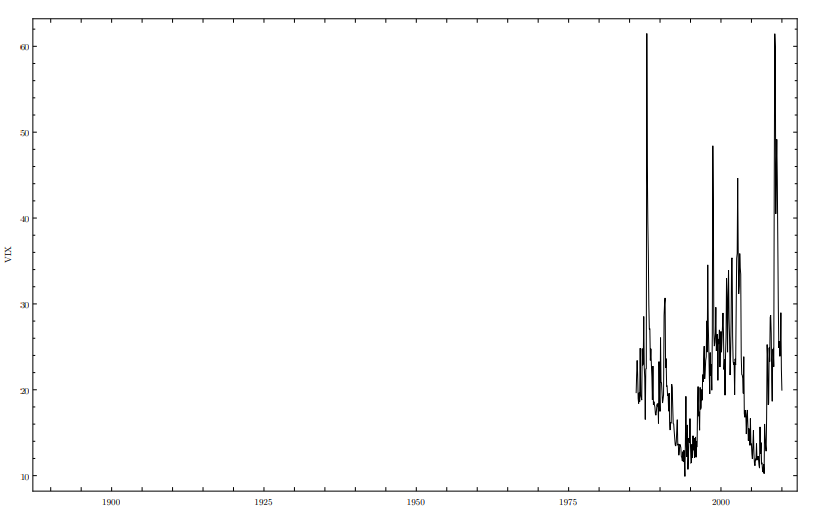
\includegraphics[scale=0.45]{Images/mm2017pre-1.png}
\end{center}
% The VIX, from 1986 onwards
\end{frame}%

\begin{frame}{\small{Manela and Moreira (2017): NVIX construction}}
\vspace{-7pt}
\begin{center}
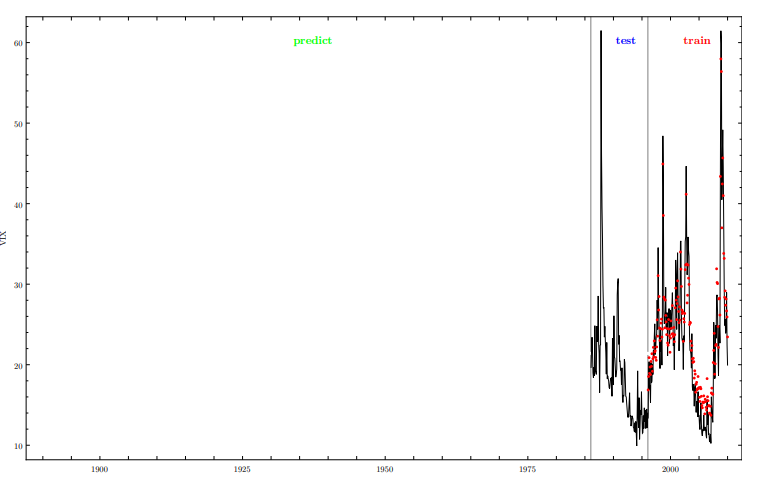
\includegraphics[scale=0.45]{Images/mm2017pre-2.png}
% The training exercise
\end{center}
\end{frame}%

\begin{frame}{\small{Manela and Moreira (2017): NVIX construction}}
\vspace{-7pt}
\begin{center}
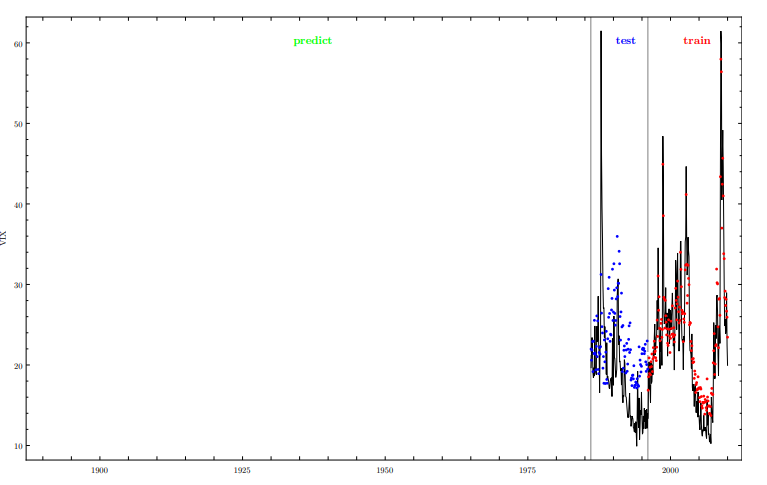
\includegraphics[scale=0.45]{Images/mm2017pre-3.png}
% The testing exercise
\end{center}
\end{frame}%

\begin{frame}{\small{Manela and Moreira (2017): NVIX construction}}
\vspace{-7pt}
\begin{center}
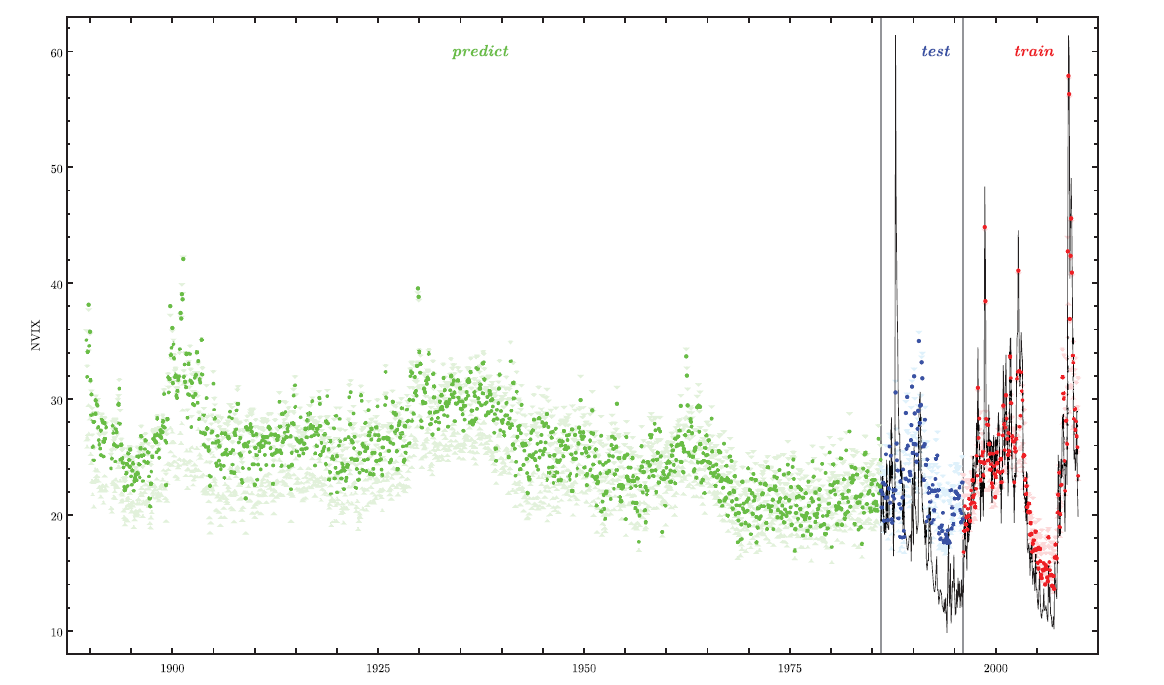
\includegraphics[scale=0.35]{Images/mm2017-1.png}
% The prediction exercise
\end{center}
\end{frame}

\begin{frame}{\small{Manela and Moreira (2017): NVIX construction}}
\vspace{-7pt}
\begin{center}
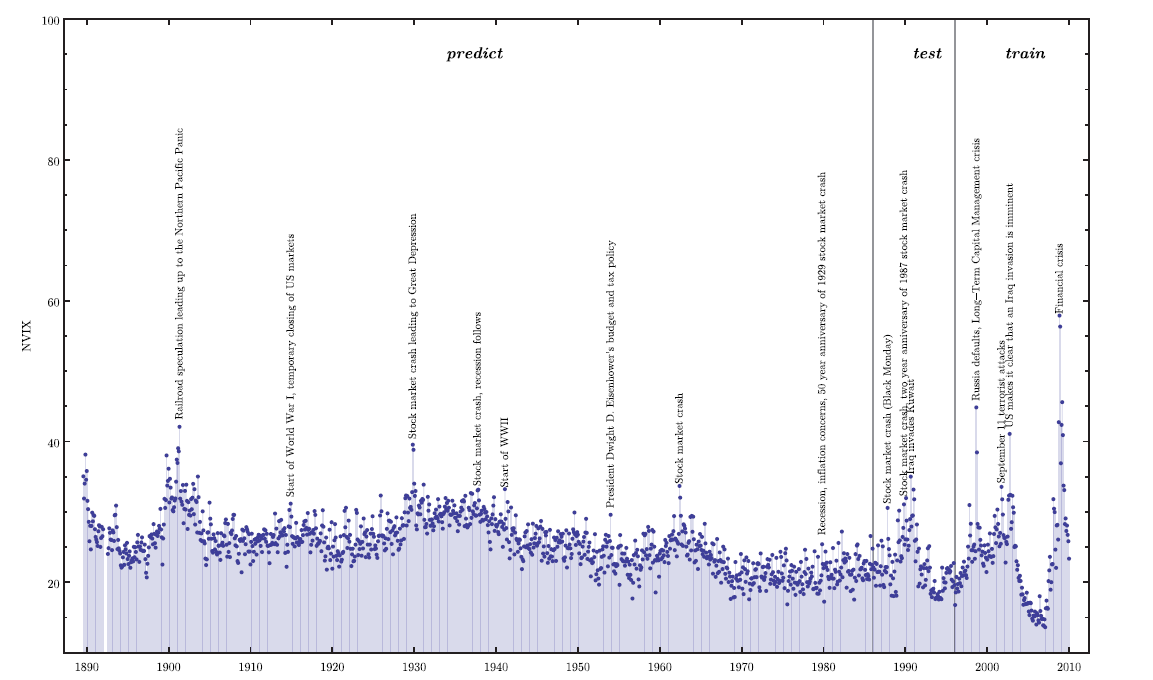
\includegraphics[scale=0.35]{Images/mm2017-2.png}
% What do they actually show
\end{center}
\end{frame}

\begin{frame}{Manela and Moreira (2017): Empirical Strategy}
\begin{itemize}
\setlength{\itemsep}{1.5em}
\item Asset pricing models with time-varying risk premia suggest that times when risk is relatively high would be followed by above average stock market returns
\\~\
\begin{itemize}
    \item Time-varying volatility (Merton, 1973)
    %Dynamic risk-return trade off predicts a linear relation between the conditional expected excess return on the market and its conditional variance
    \item Time-varying disaster risk (Gabaix, 2012)
    %More recent models predict a linear relation between expected excess returns and the variance premium, which is linear in the time-varying probability of a rare disaster.
\end{itemize}
\item Goal: explain future excess return on the market protfolio at various horizons with lagged forward-looking measures of risk as measured by NVIX squared
% The overarching hypothesis is that time variation in uncertainty is an important driver of variation in expected returns on US equity. 
\end{itemize}
\end{frame}%

\begin{frame}{\small{Manela and Moreira (2017): Estimation Results}}
\vspace{-7pt}
\begin{center}
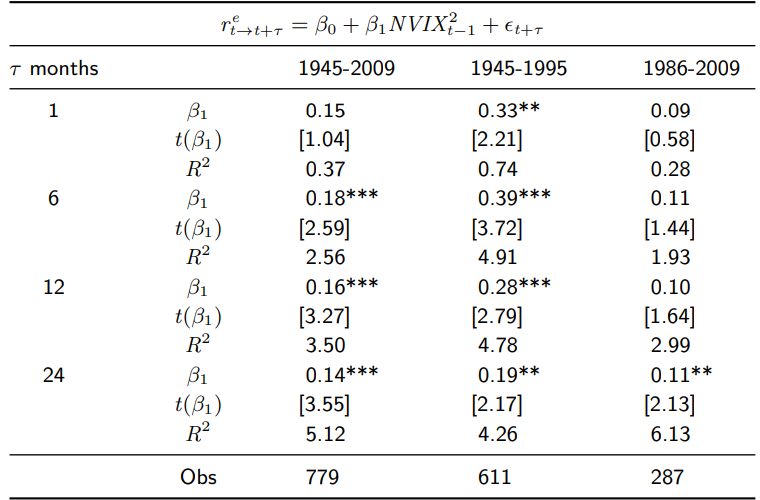
\includegraphics[scale=0.5]{Images/mm2017-3.png}
% To prove the above, they try to explain future excess returns on the market portfolio at various horizons with lagged forward-looking variables of risk as measured by NVIX squared. 
\end{center}
\end{frame}

\begin{frame}{Supervised machine learning}
\begin{itemize}
\setlength{\itemsep}{1.2em}
\setlength{\itemindent}{-0.8em}
\item \textcolor{blue}{Goal}: classify documents into pre-existing categories

\item \textcolor{blue}{What do we need}: 
\vspace{4pt}
\begin{itemize}
\setlength{\itemindent}{-1.5em}
\setlength{\itemsep}{0.5em}
\item Hand-coded labeled dataset, to be split into \textcolor{blue}{training} set and a\\
\hspace{-14pt}\textcolor{blue}{validation/test set}
\item Method to extrapolate from hand-coding to unlabeled, i.e., \textcolor{blue}{classifier}
\end{itemize}

\item Possible classifiers:
\vspace{4pt}
\begin{itemize}
\setlength{\itemindent}{-1.5em}
\setlength{\itemsep}{0.5em}
\item \textcolor{blue}{Regularized regressions}
\item \textcolor{blue}{Naive Bayes}
\item Support Vector Machines
\item Ensemble classifiers
\end{itemize}
 
\end{itemize}
\end{frame}

\begin{frame}{Supervised machine learning}
\begin{itemize}
\setlength{\itemsep}{1.2em}
\setlength{\itemindent}{-0.8em}
\item \textcolor{blue}{Goal}: classify documents into pre-existing categories

\item \textcolor{blue}{What do we need}: 
\vspace{4pt}
\begin{itemize}
\setlength{\itemindent}{-1.5em}
\setlength{\itemsep}{0.5em}
\item Hand-coded labeled dataset, to be split into \textcolor{blue}{training} set and a\\
\hspace{-14pt}\textcolor{blue}{validation/test set}
\item Method to extrapolate from hand-coding to unlabeled, i.e., \textcolor{blue}{classifier}
\end{itemize}

\item Possible classifiers:
\vspace{4pt}
\begin{itemize}
\setlength{\itemindent}{-1.5em}
\setlength{\itemsep}{0.5em}
\item \textcolor{blue}{Regularized regressions}
\item \textcolor{blue}{Naive Bayes}
\item Support Vector Machines
\item Ensemble classifiers
\end{itemize}
 
\end{itemize}
\end{frame}

\begin{frame}{Stock-Trebbi 2003: who invented instrumental variables?}
\begin{itemize}
\setlength{\itemsep}{0.7em}
\item First derivation of IV estimator in Appendix B of \textit{The Tariff on Animal and Vegetable Oils} by Philip G. Wright (1928)

\vspace{5pt}

\begin{itemize}
\setlength{\itemsep}{0.5em}
\item First 285 pages: ``a painfully detailed treatise on animal and vegetable oils, their production, uses, markets and tariffs''
\item Appendix B: ``Out of the blue... a succinct and insightful of why price and quantity data alone are in general inadequate, two separate and correct derivations of IV, and an empirical application to butter and flaxseed''
\end{itemize}
 \item Because Appendix B is so different many people (e.g., Manski 1988) have suggested it might have been written by Philip's son Sewall Wright, a famous genetic statistician
\end{itemize}
\end{frame}

\begin{frame}{}
\begin{center}
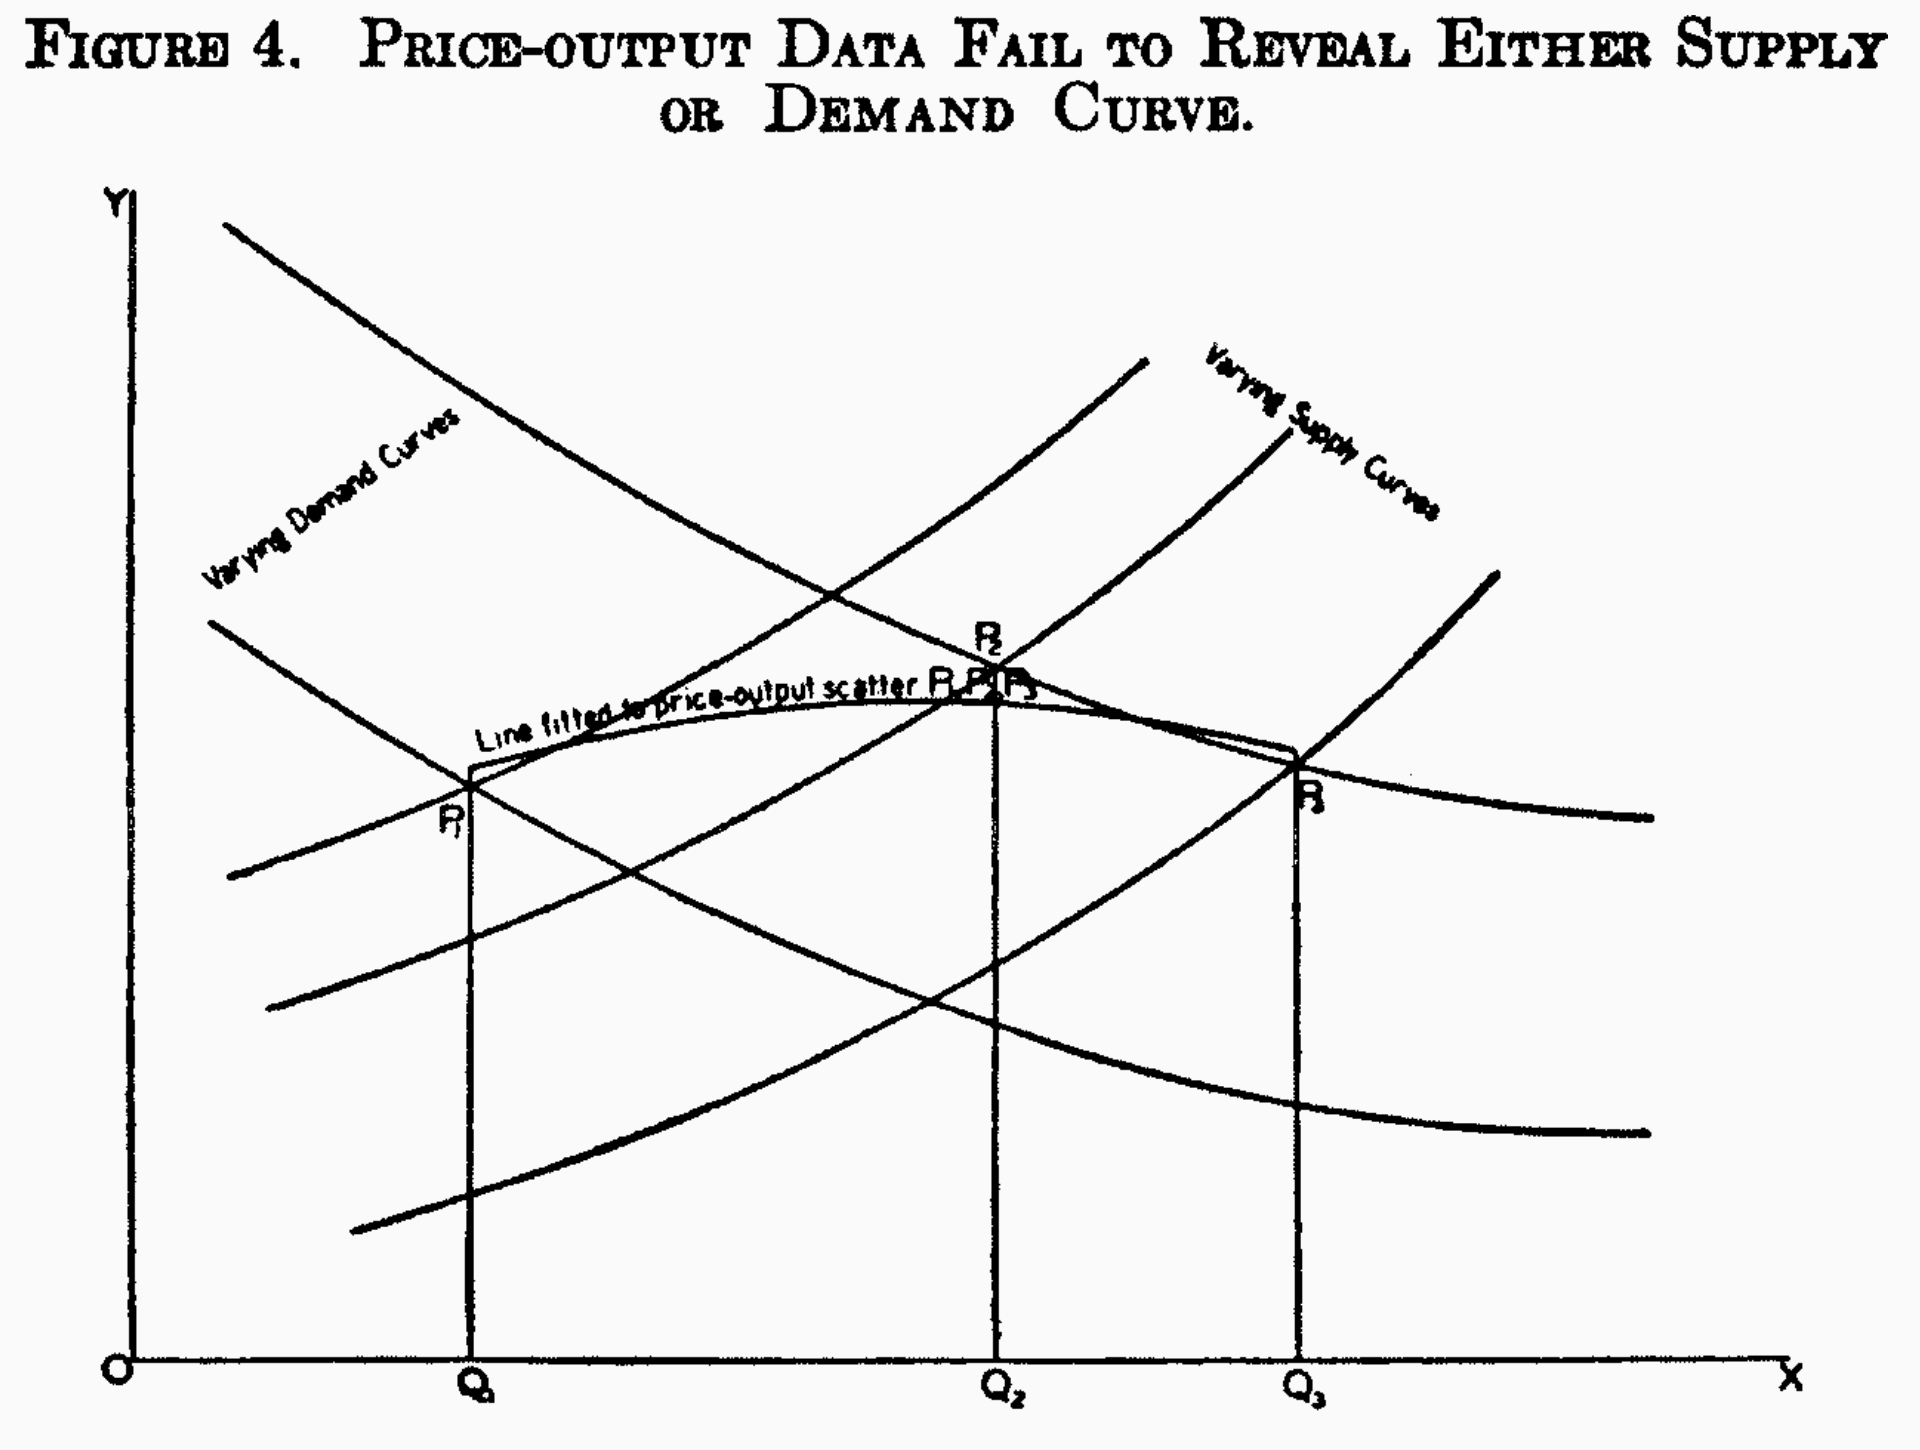
\includegraphics[width=1 \textwidth]{Images/fischer_graph1.png}
\end{center}
\end{frame}

\begin{frame}{Authorship debate}
\begin{itemize}
\setlength{\itemsep}{1.5em}
    \item Case for Sewall:
    \vspace{5pt}
    \begin{itemize}
        \setlength{\itemsep}{0.7em}
        \item Appendix uses method of ``path coefficients'' which Sewall had recently invented
        \item A more eminent statitician
    \end{itemize}
    \item Case for Philip:
    \vspace{5pt}
    \begin{itemize}
        \setlength{\itemsep}{0.7em}
        \item Was an economist while Sewall was not
        \item Had written frequently about the identification problem
    \end{itemize}
\end{itemize}
\end{frame}

\begin{frame}{Sample}
\begin{itemize}
\setlength{\itemsep}{1.5em}
\item Each ``document'' is a block of 1000 words 
\item ``Training set''
    \vspace{5pt}
\begin{itemize}
\setlength{\itemsep}{0.4em}
\item 20 undisputedly by Sewall
\item 25 undisputedly by Philip
    \end{itemize}
    \item ``Prediction set''
        \vspace{5pt}
    \begin{itemize}
        \item 6 from Appendix B
        \item 1 from Chapter 1
    \end{itemize}
\end{itemize}
\end{frame}

\begin{frame}{From text to data}
\begin{itemize}
\setlength{\itemsep}{1.4em}
\item Define columns of $C$ to be:
        \vspace{5pt}
\begin{itemize}
\setlength{\itemsep}{0.4em}
\item Counts of 70 ``function words'' taken from Mosteller \& Wallace
\item Counts of 18 ``grammatical constructions'' from Mannion \& Dixon (1997)
\end{itemize}
\item Result: $n = 52$, $p = 88$, with $V$ observed for 45 documents
\end{itemize}
\end{frame}

\begin{frame}{}
\centering
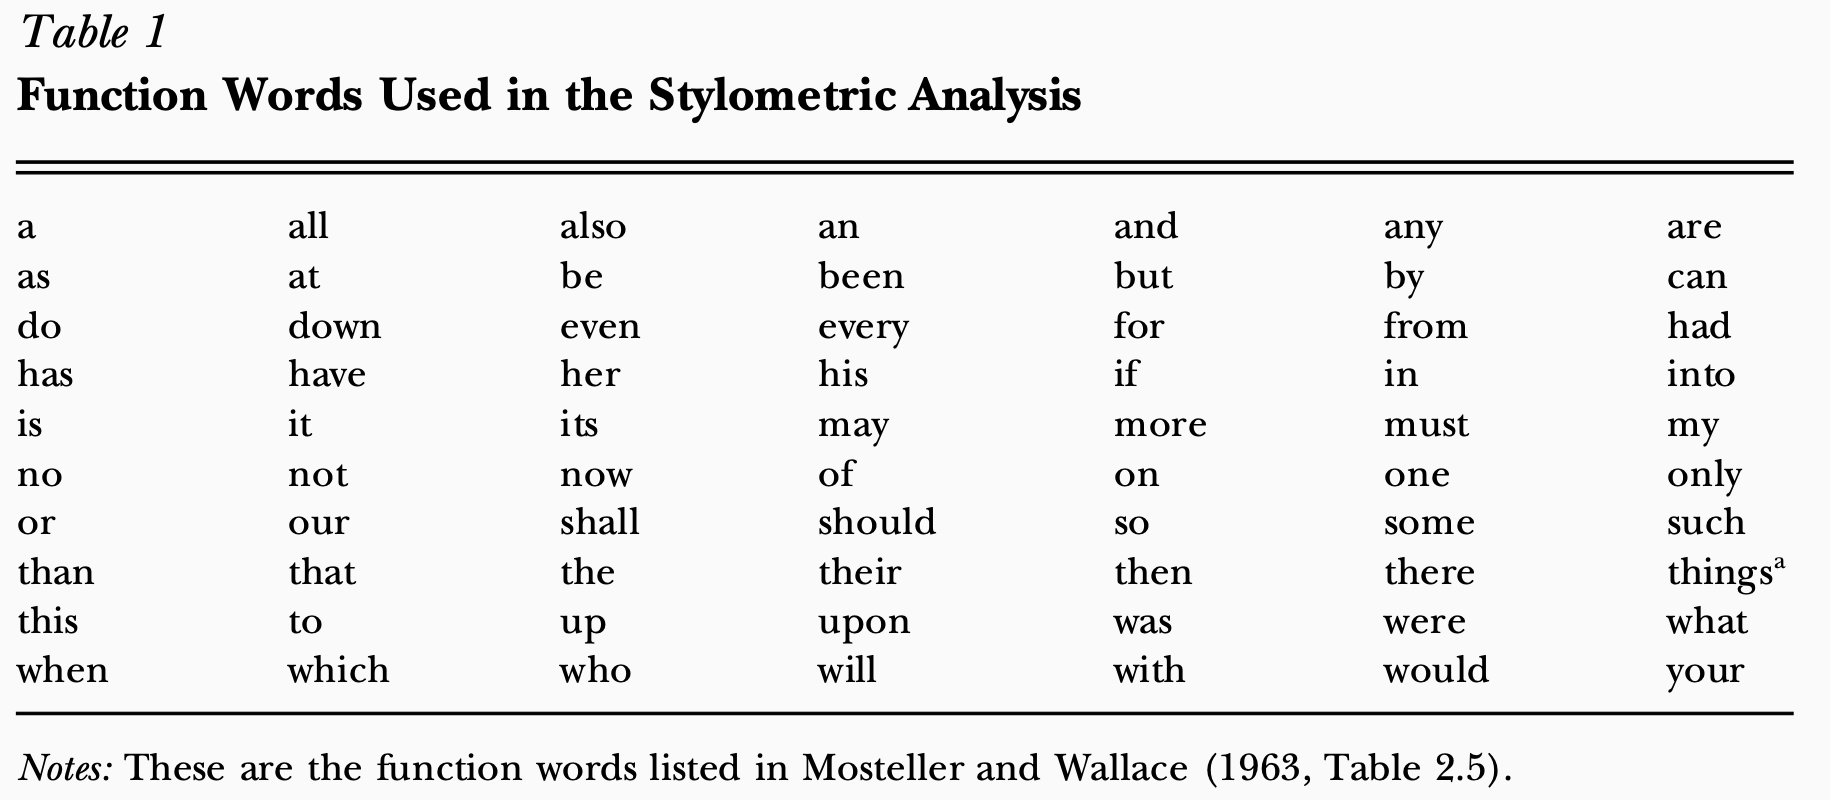
\includegraphics[width=1 \textwidth]{Images/fischer_table1.png}
\end{frame}

\begin{frame}{}
\centering
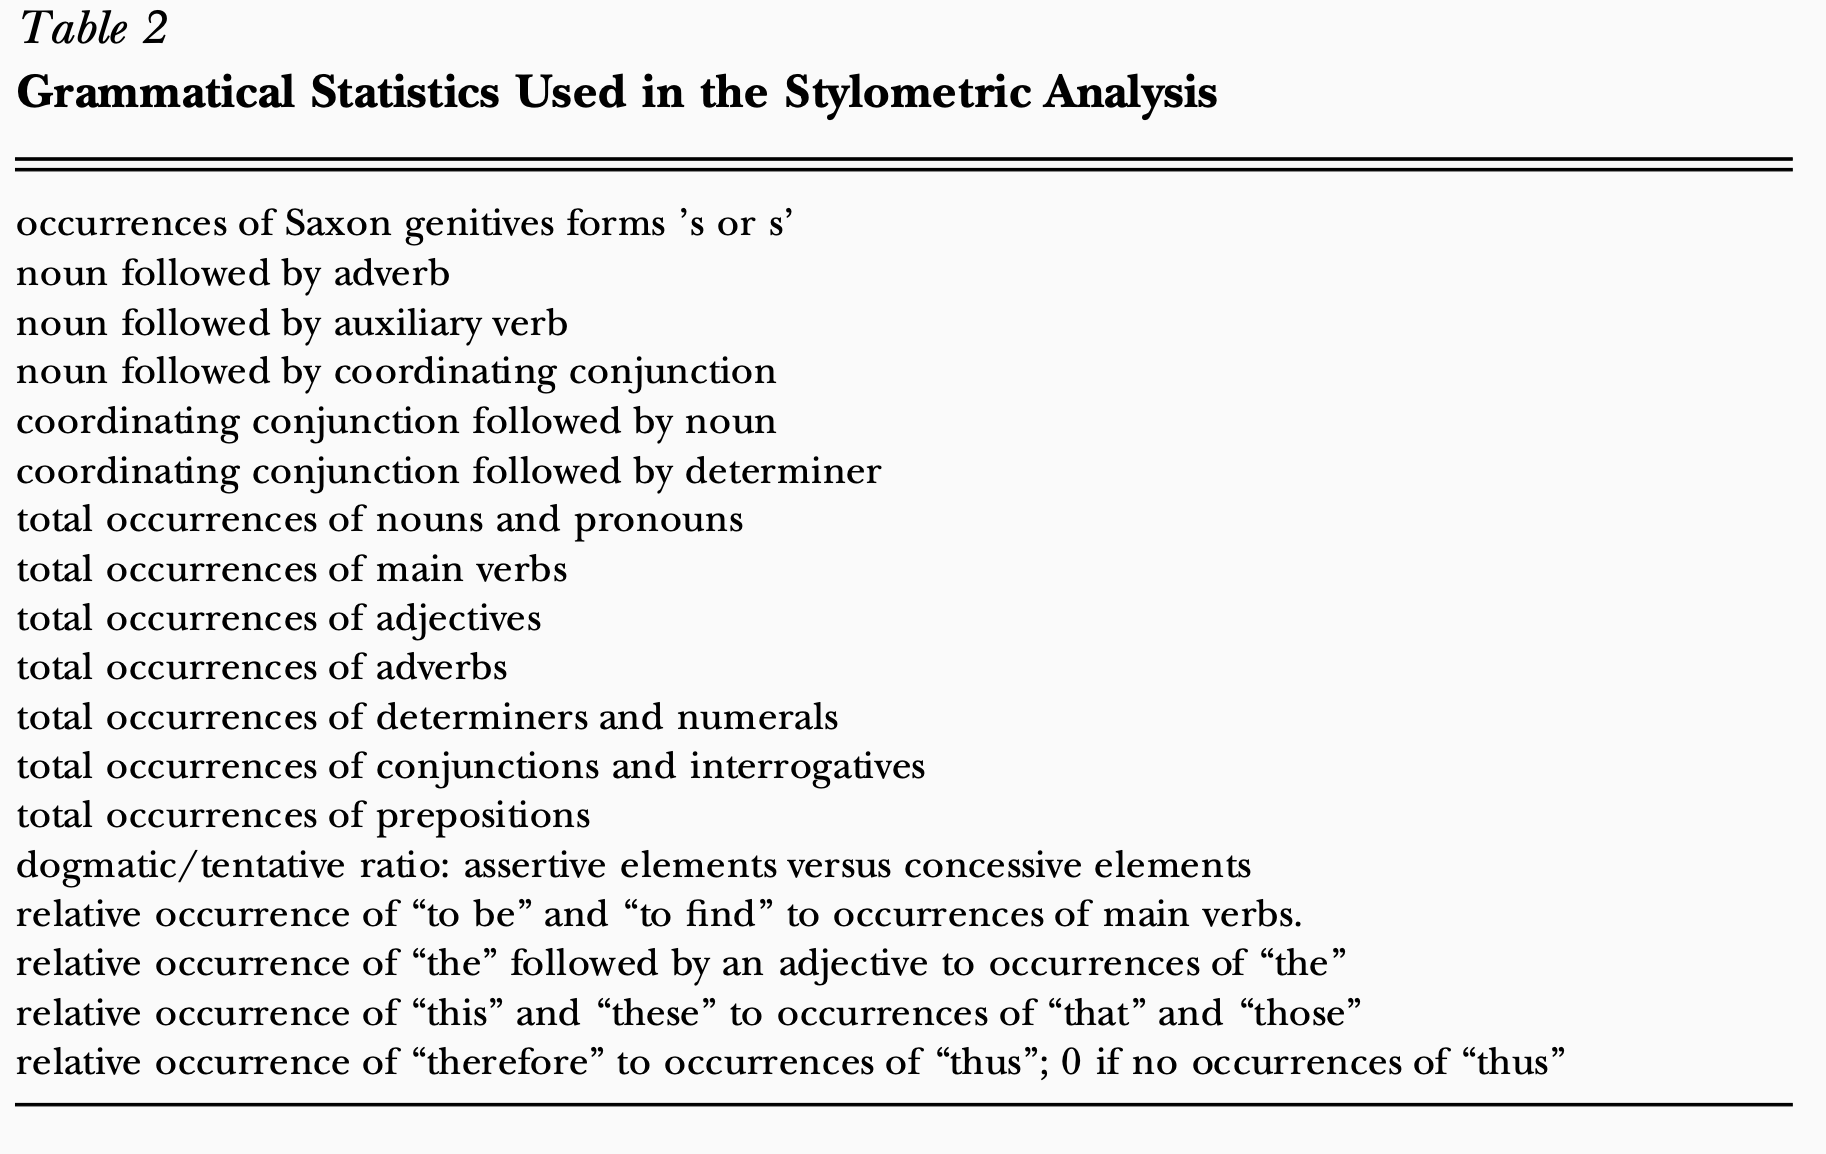
\includegraphics[width=1 \textwidth]{Images/fischer_table2.png}
\end{frame}

\begin{frame}{Method}
\begin{itemize}
\item We still have $p>n$, so just regressing $V$ on $c$ is unfeasible
\item Two measures, each computed for function words and grammar separately, to produce $(\hat{V}_{fw}, \hat{V}_{g})$
\end{itemize}
\end{frame}

\begin{frame}{Approach \#1: PCA}
\begin{itemize}
    \item Compute 4 principal components of $C_{fw}$ and $C_g$
    \item Regress $V$ on each separately
    \item (Unsupervised dimension reduction)
\end{itemize}
\end{frame}

\begin{frame}{Approach \#1: linear discriminant analysis (Fischer, 1936)}
\begin{itemize}
    \item Compute ``linear discriminant'' of $C_{fw}$ and $C_g$ 
    \end{itemize}
    \vspace{15pt}
    \centering
    \large $\hat{V} = \sum_{p}{w_p c_p}$ \\
    \vspace{15pt}
    \centering
    \large $w_{p} = \frac{\bar{C}_{p:P} - \bar{C}_{p:S}}{s_{p:P}^{2} + s_{p:S}^{2}}$
    \vspace{15pt}
\begin{itemize}
\setlength{\itemsep}{0.7em}
\item This is the optimal Bayes classifier if X's are normal with equal variance
\item Supervised dimension reduction using generative model
\end{itemize}
\end{frame}

\begin{frame}{}
\centering
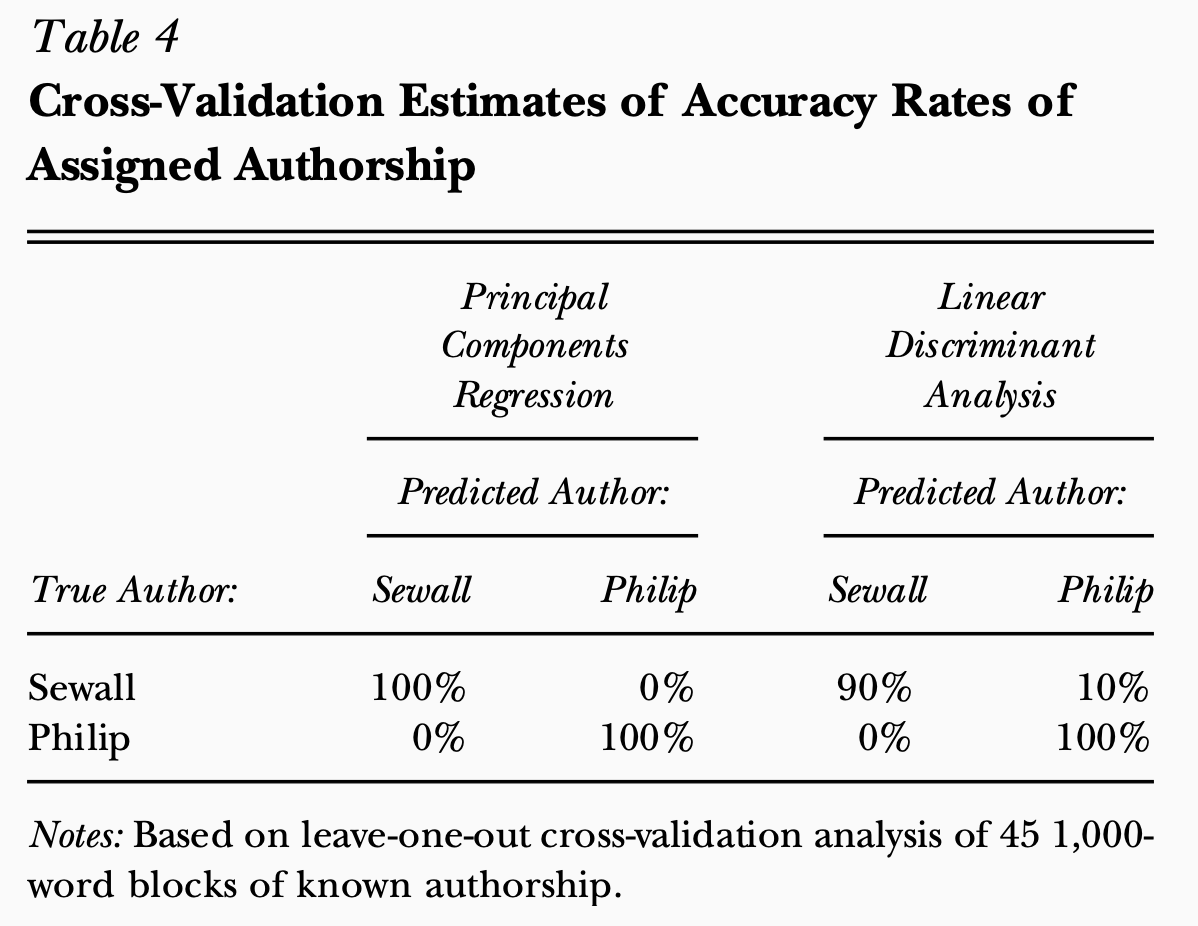
\includegraphics[width=0.9 \textwidth]{Images/fischer_table4.png}
\end{frame}

\begin{frame}{}
\centering
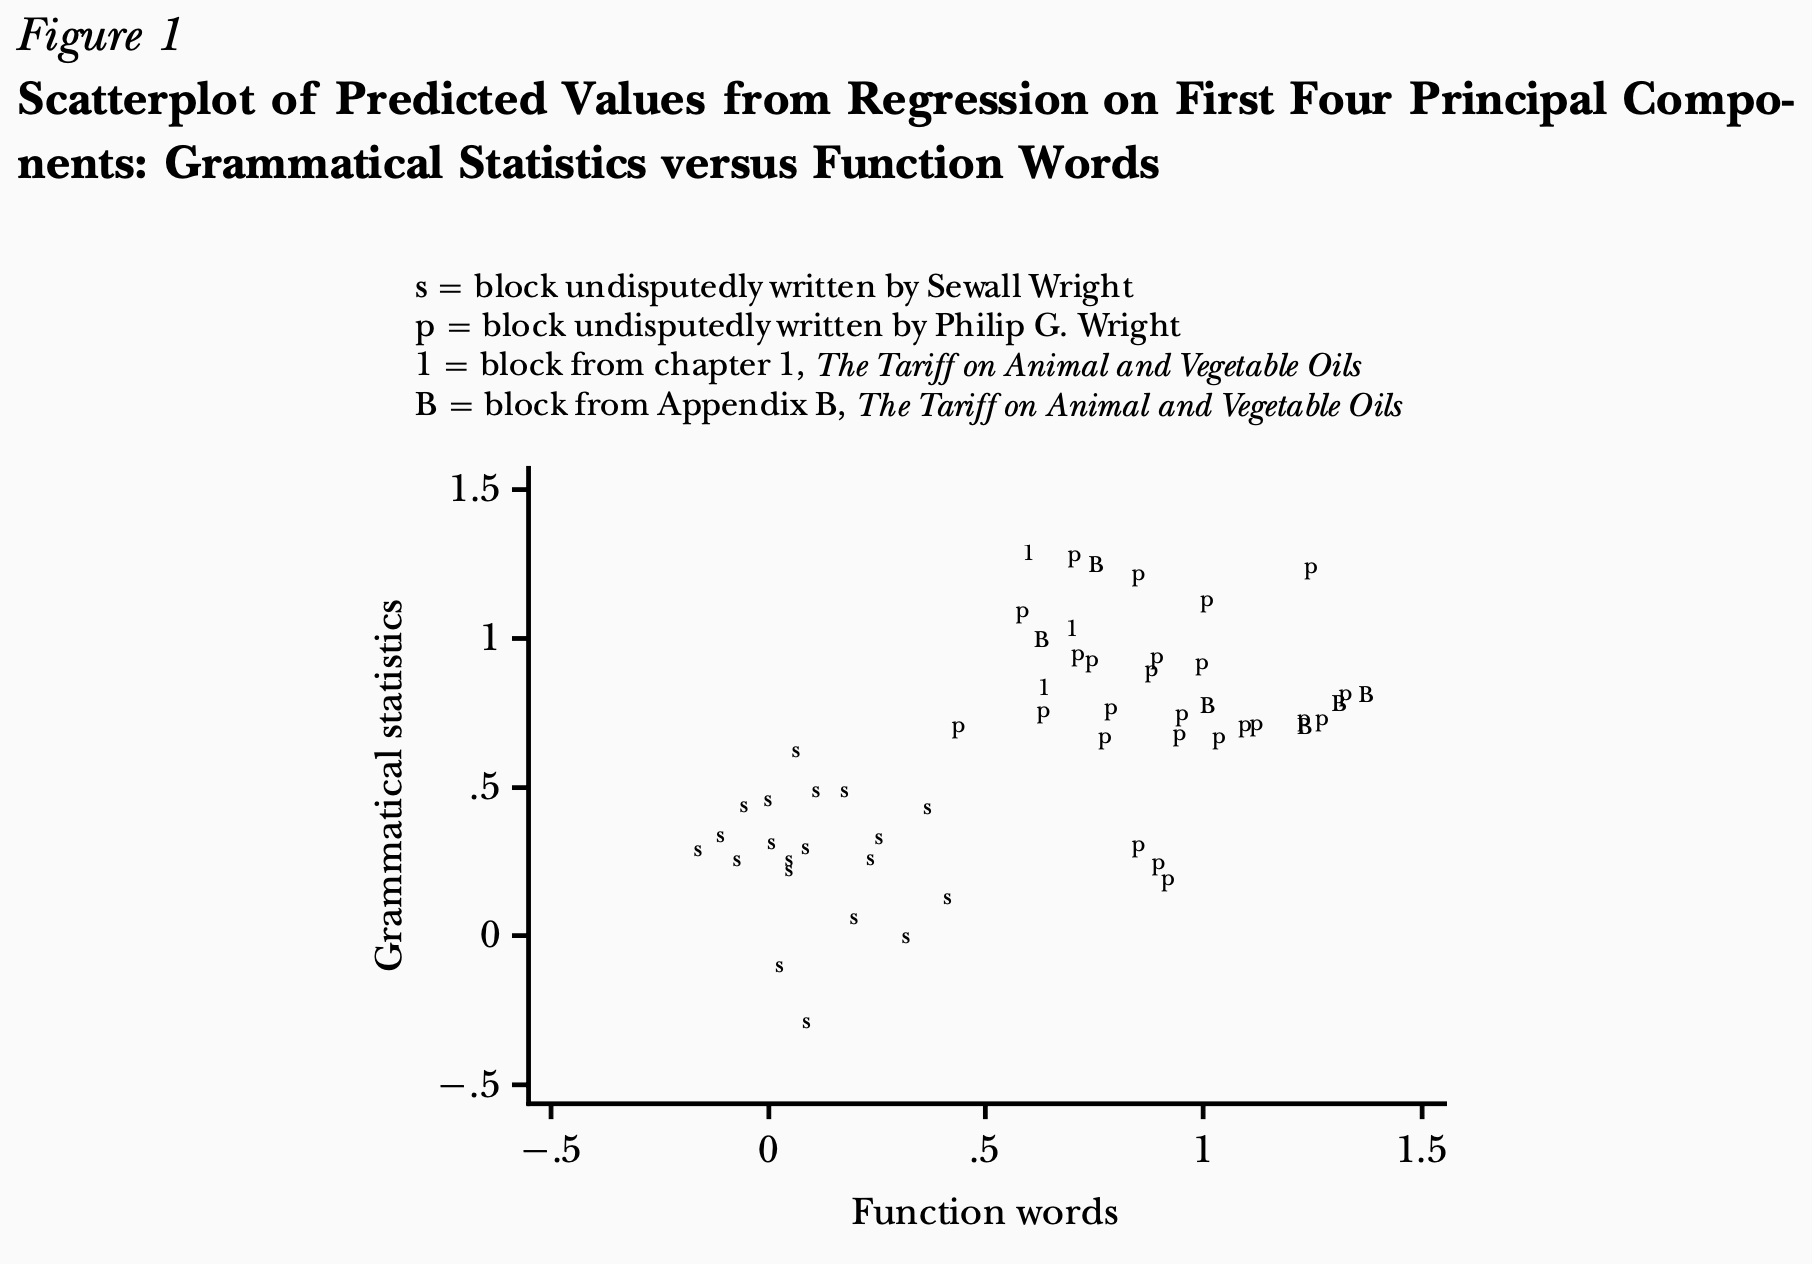
\includegraphics[width=1 \textwidth]{Images/fischer_figure1.png}
\end{frame}

\begin{frame}{}
\centering
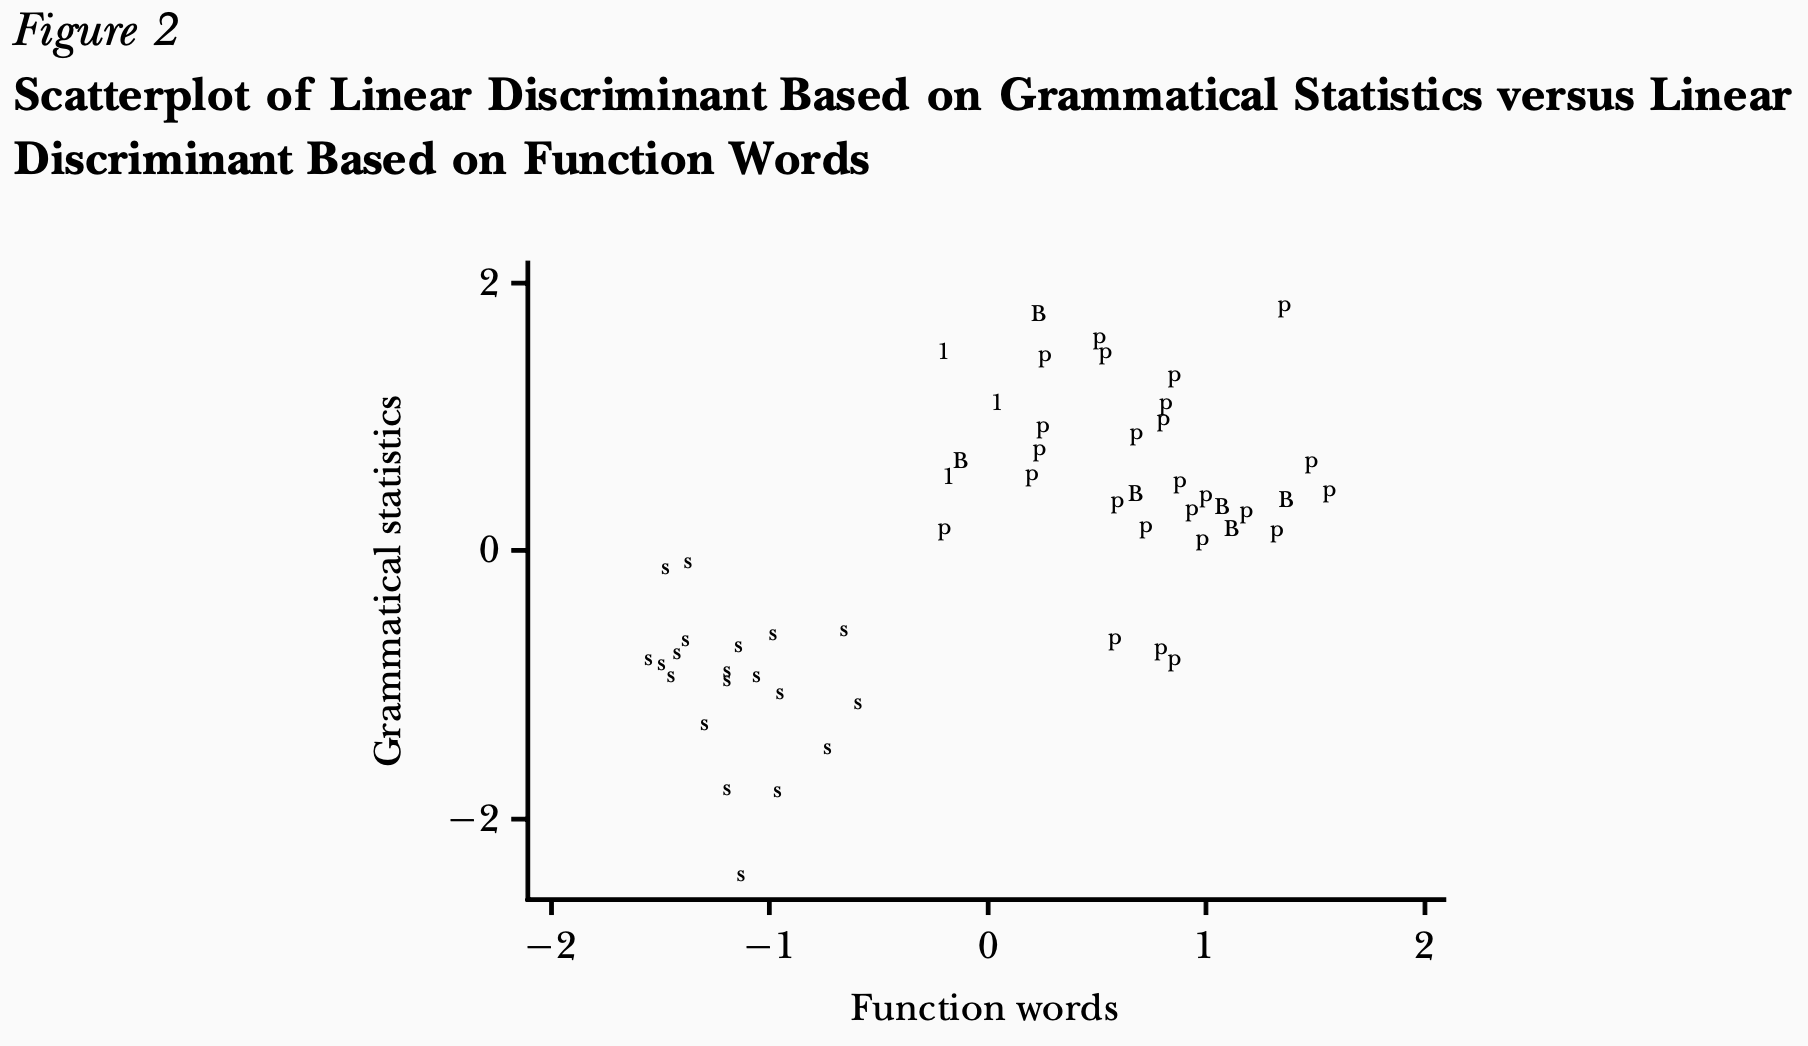
\includegraphics[width=1 \textwidth]{Images/fischer_figure2.png}
\end{frame}

\begin{frame}{Conclusion}
\setlength{\itemsep}{0.7em}
\begin{itemize}
\item Philip is undoubtedly the author
 \item Of course this didn't mean it was his \textit{idea}
\item But Stock \& Trebbi conclude it probably was
\end{itemize}
\end{frame}

\begin{frame}{Financial news and asset price: Antweiler-Frank 2004}
\begin{itemize}
\item Data: Message board contents on Yahoo!Finance \& Raging Bull
\end{itemize}
\vspace{10pt}
\centering
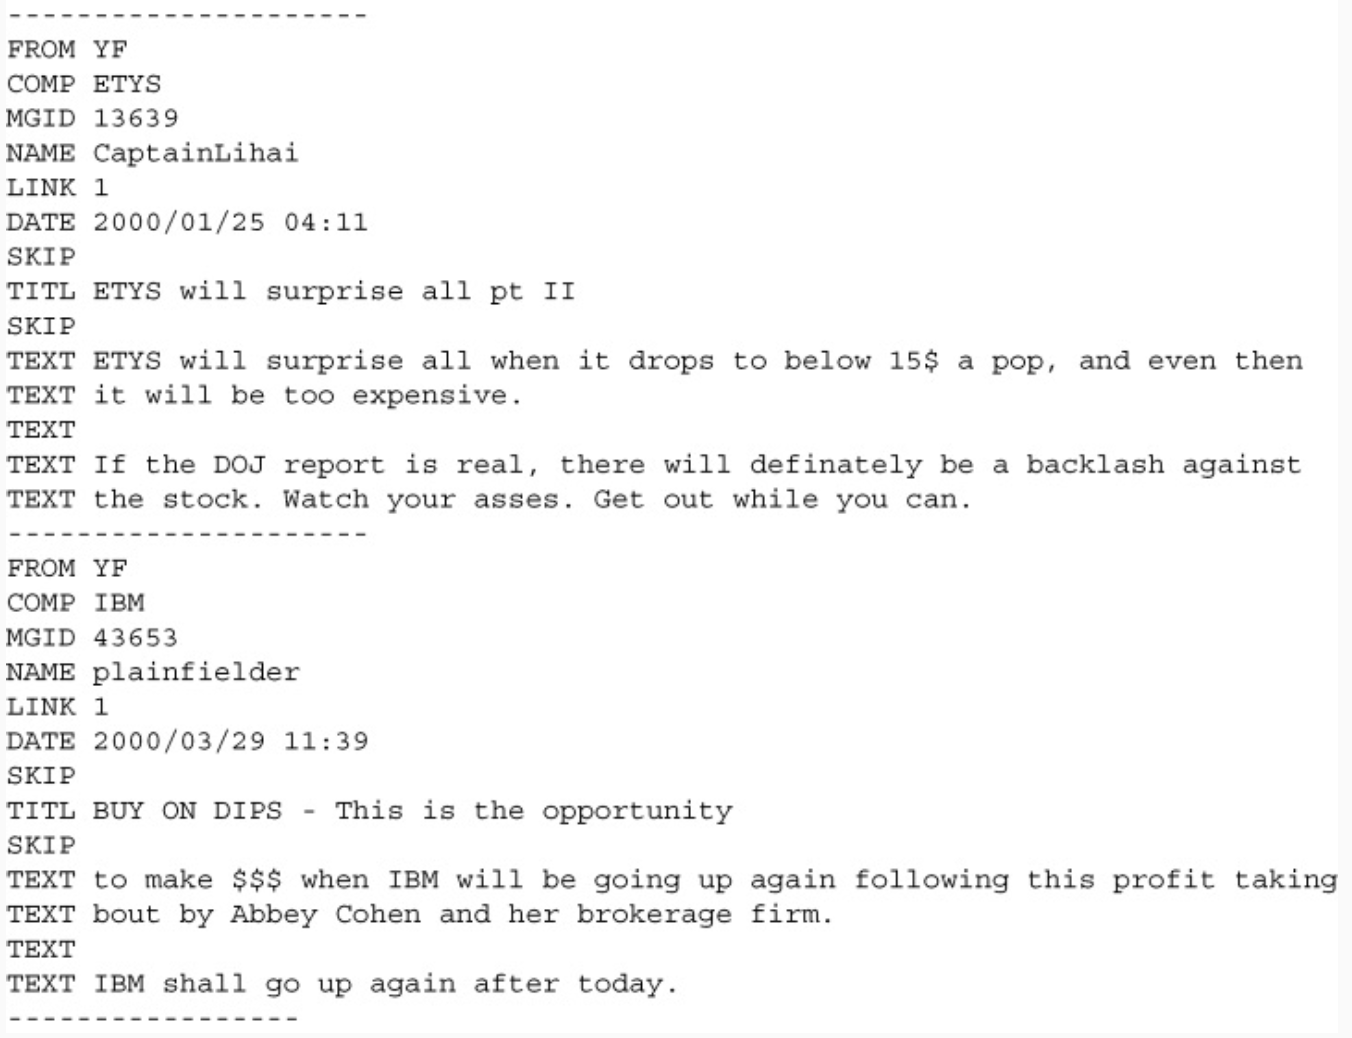
\includegraphics[width=0.75 \textwidth]{Images/antfrank1.png}
\end{frame}

\begin{frame}{Antweiler and Frank 2004}
\begin{itemize}
\setlength{\itemsep}{0.7em}
\item Count words
\item Create training set of 1,000 messages hand-coded as: buy, sell, hold
\item Compute ``naive Bayes classification:'' posterior guess assuming words are independent
\end{itemize}
\centering
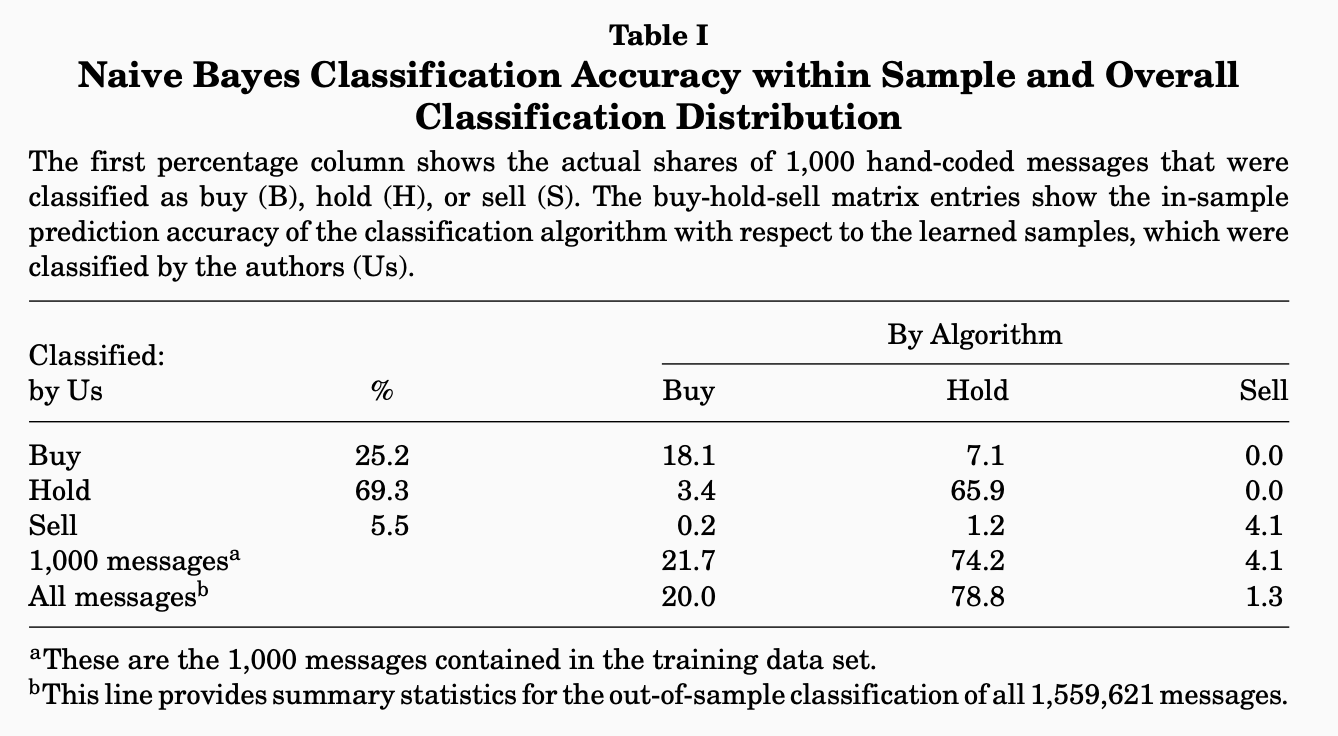
\includegraphics[width=0.85 \textwidth]{Images/antfrank2.png}
\end{frame}

% Posterior given the data under the assumption that words are independent from each other

\begin{frame}{Antweiler and Frank 2004}
\begin{itemize}
\setlength{\itemsep}{1em}
    \item Small amount of predictability in returns
    \item Messages predict volatility
    \item Disagreement (variable recommendations) predicts volume
\end{itemize}
\end{frame}

\begin{frame}{Research question}
\begin{itemize}
\setlength{\itemsep}{0.85em}
\item How to measure partisan bias in the media?

\pause

\item{Mass media can \textcolor{blue}{slant} the news to favor a particular point of view (\textit{partisan bias})}

\pause

\item{Forms of partisan bias:


\vspace{7pt}

\begin{itemize}
\setlength{\itemindent}{-1em}
\setlength{\itemsep}{0.4em}
\item{Unbalanced reporting of political events (language, citations, etc.)}
\vspace*{4pt}
\item{More newstime devoted to like-minded politicians/experts}
\vspace*{4pt}
\item{More emphasis on issues on which a party is perceived as stronger}
\vspace*{4pt}
\item{More emphasis on bad performance or scandals of opposing party}
\end{itemize}}

\item In any case, a very elusive object!

\pause

\item Important to study other questions, e.g., what drives media bias?

\end{itemize}

\end{frame}


\begin{frame}

\frametitle{Media bias: an example}

\begin{itemize}
\item \textcolor{blue}{Fox News}:\\
\vspace{2pt}
%\begin{itemize}
\textit{``In one of the deadliest reported firefights in Iraq since the fall of Saddam Hussein's regime, US forces killed at least 54 Iraqis and captured eight others while fending off simultaneous convoy ambushes Sunday in the northern city of Samarra.''}
%\end{itemize}
\end{itemize}

\vspace{3pt}

\begin{itemize}
\item \textcolor{blue}{New York Times}:\\
\vspace{3pt}
%\begin{itemize}
\textit{``American commanders vowed Monday that the killing of as many as 54 insurgents in this central Iraqi town would serve as a lesson to those fighting the United States, but Iraqis disputed the death toll and said anger against America would only rise.''}
%\end{itemize}
\end{itemize}

\vspace{3pt}

\begin{itemize}
\item \textcolor{blue}{Al-Jazeera.net}:\\
\vspace{2pt}
%\begin{itemize}
\textit{``The US military has vowed to continue aggressive tactics after saying it killed 54 Iraqis following an ambush, but commanders admitted they had no proof to back up their claims. The only corpses at Samarra's hospital were those of civilians, including two elderly Iranian visitors and a child.''}
%\end{itemize}
\end{itemize}

\end{frame}

\begin{frame}

\frametitle{A Measure of Media Bias (Groseclose-Milyo, 2005)}

\begin{itemize}
\setlength{\itemsep}{0.9em}

\item{\textcolor{blue}{\large Goal:}
\vspace*{5pt}
\begin{itemize}
\setlength{\itemsep}{0.5em}
\setlength{\itemindent}{-1em}
\item{Estimate relative ideological scores for several major U.S. media outlets}
\end{itemize}}

\pause

\item{\textcolor{blue}{\large Empirical Idea:}
\vspace*{5pt}
\begin{itemize}
\setlength{\itemsep}{0.5em}
\setlength{\itemindent}{-1em}
\item{Count the times a media outlet cites various think tanks and compare\\
\hspace{-9pt}with the times members of Congress cite the same groups}
\item{Citations are the language, politicians the reference point}
\item{Only look at content (no editorials, letters, etc.)}
\end{itemize}}

\pause

\item{\textcolor{blue}{\large Findings:}
\vspace*{5pt}
\begin{itemize}
\setlength{\itemsep}{0.5em}
\setlength{\itemindent}{-1em}
\item{Strong liberal bias: all news outlets but two (Fox News, Washington\\
\hspace{-10pt}Times) have scores to the left of the average member of Congress}
\item{Most leftist: CBS Evening News, NYT}
\item{Most centrist: PBS NewsHour, CNN's Newsnight, ABC's Good\\
\hspace{-10pt}Morning America, USA Today}
\end{itemize}}
\end{itemize}
\end{frame}

\begin{frame}

\frametitle{Data}

\begin{itemize}
\setlength{\itemsep}{0.4em}
\item{\small List of 200 of the most prominent US think tanks and policy groups}
\vspace*{3pt}
\item{\small Search the \textit{Congressional Record} for instances where a member of Congress cited one
of these think tanks (from 1993 to 2002)}
\vspace*{3pt}
\item{\small Record the average (adjusted) ADA score of the member who cited \\
the think tank (0-conservative to 100-liberal).}
\pause
\vspace*{3pt}
\item{\small Include citations in written reports.}
\vspace*{3pt}
\item{\small Do not consider mentions of actions, but just views of the TT/PG.}
\vspace*{3pt}
\item{\small Omit cases where a politician/media outlet mentions a TT/PG just to criticize it (only 5\% and 1\% of mentions respectively)}
\vspace*{3pt}
\item{\small Omit cases where a politician/media gave an ideological label to a TT/PG (only 2\% and 5\% respectively}
\vspace*{3pt}
\pause
\item{\small ``The idea is that we only wanted cases where the legislator/journalist cited the think tank as if it were a disinterested expert on the topic''}
\end{itemize}
\end{frame}

\begin{frame}
\frametitle{Think Tanks}
\vspace{-10pt}
\begin{center}
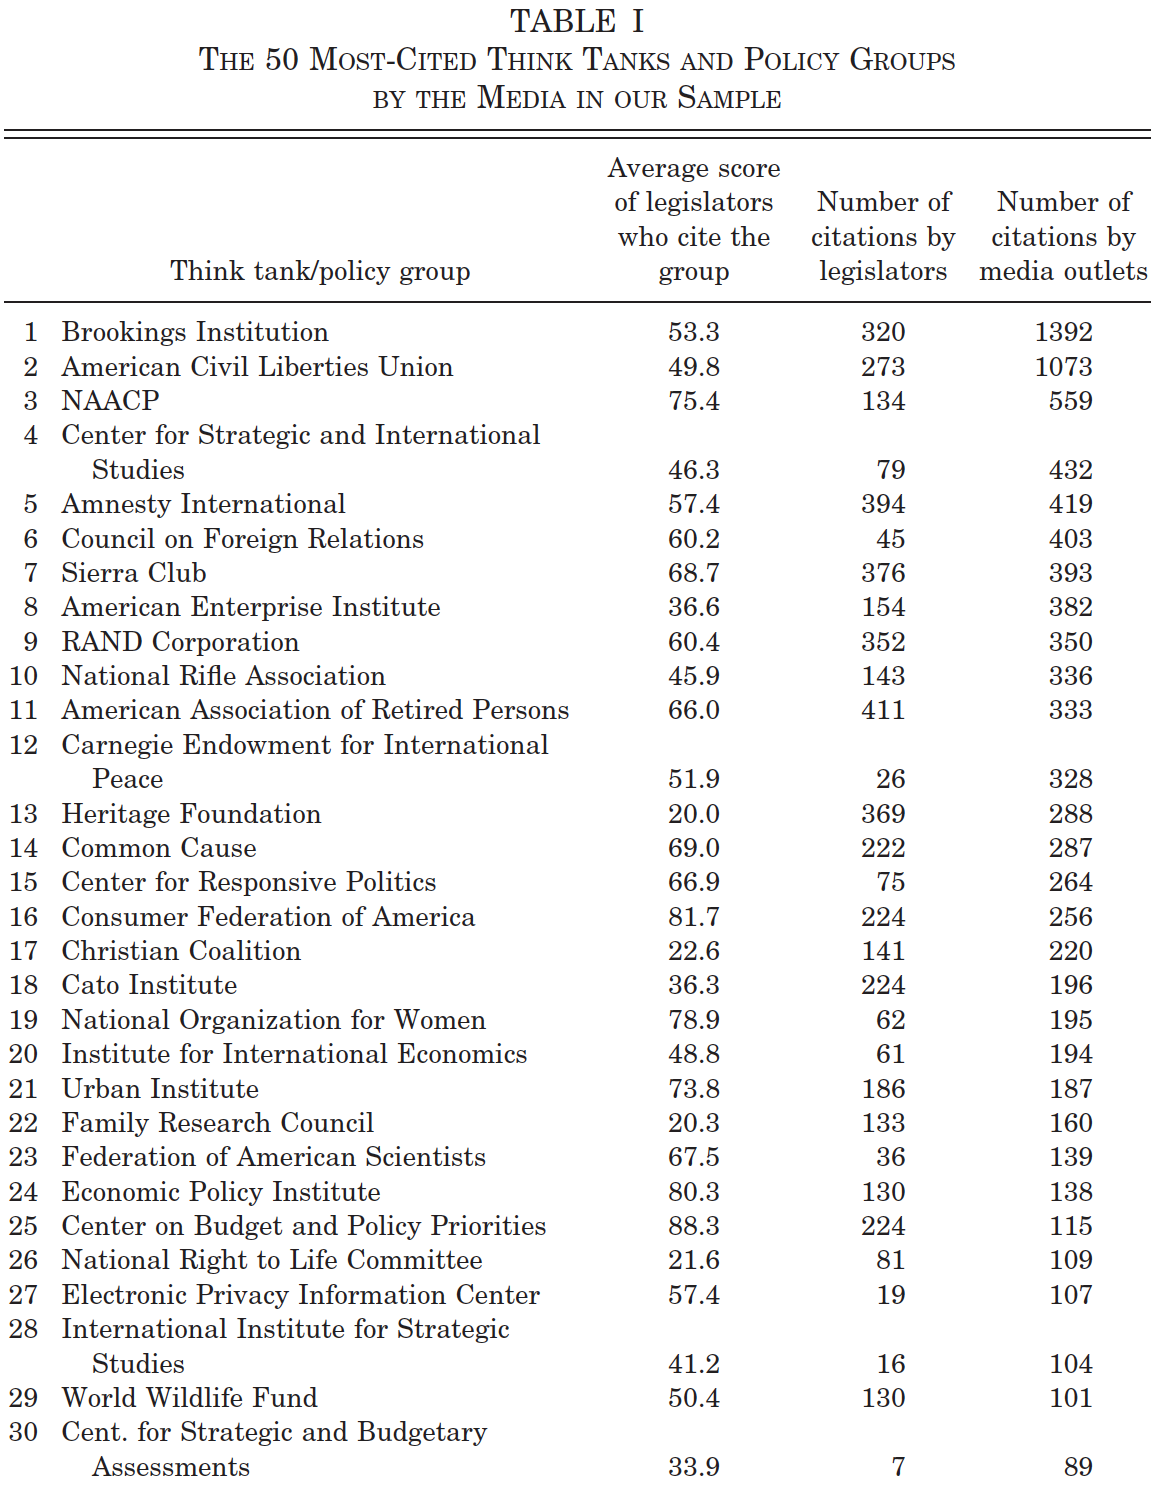
\includegraphics[scale=0.33]{Images/groseclose_milyio_table3}
\end{center}
\end{frame}

\begin{frame}
\frametitle{Politicians}
\vspace{-10pt}
\begin{center}
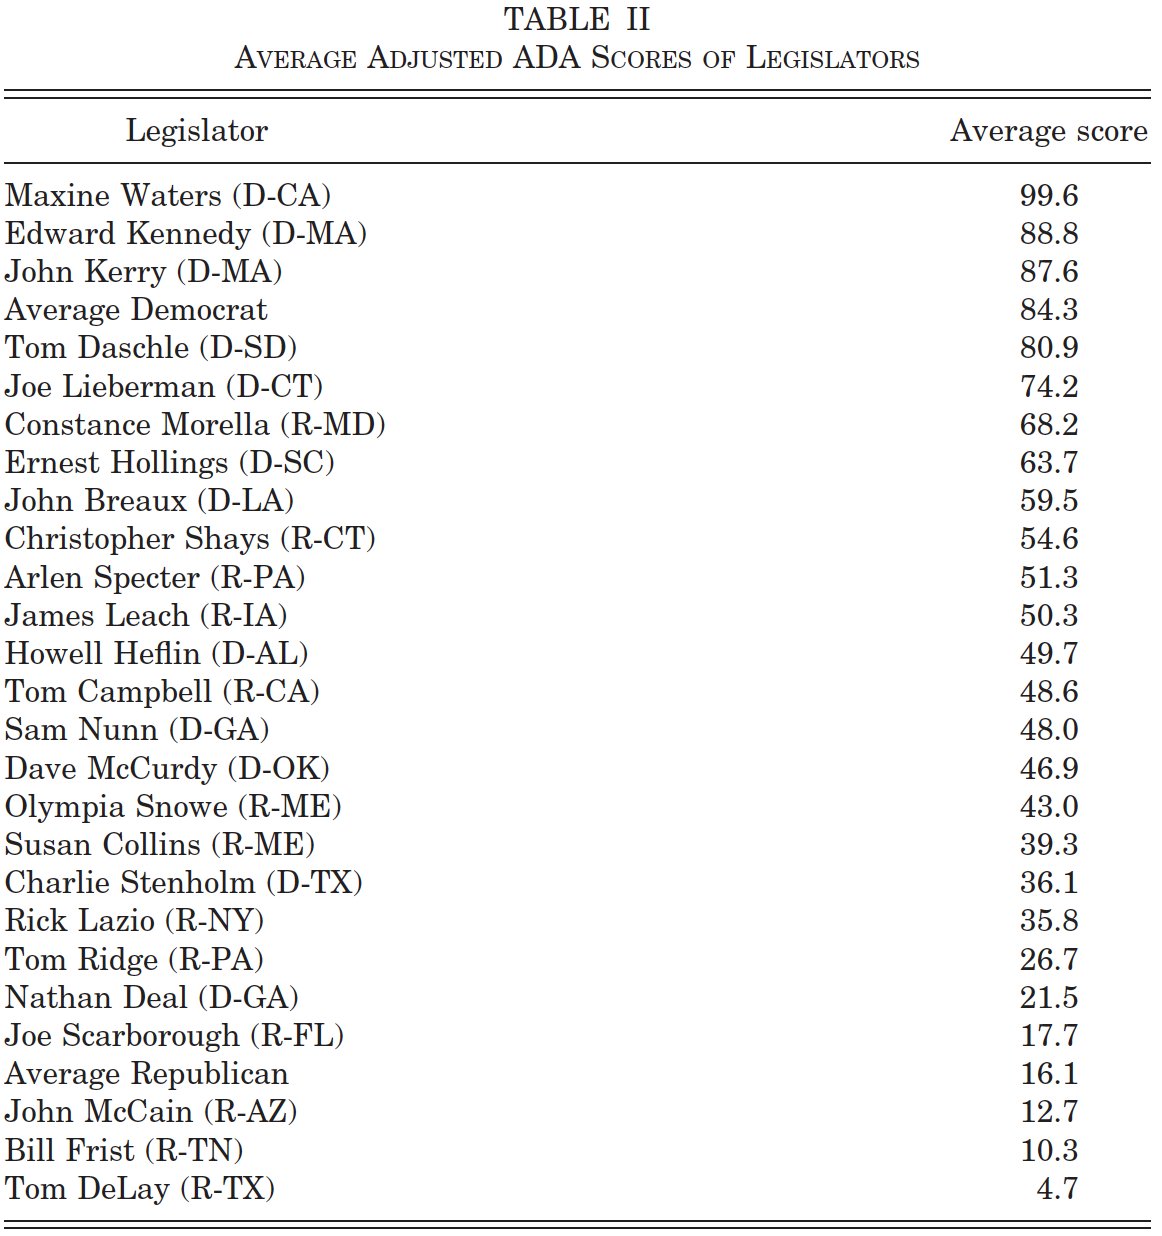
\includegraphics[scale=0.39]{Images/groseclose_milyio_table4}
\end{center}
\end{frame}


\begin{frame}

\frametitle{Definition of Bias}

\begin{itemize}
\item{Nothing to do with honesty or accuracy; more like a preference}
\vspace*{7pt}
\item{The centrist US voter in the late 1990s had a left-right ideology approximately equal to Specter (R-PA; 51.3) or Nunn (D-GA; 48.0)}
\vspace*{7pt}
\item{The average NYT article has an ideology approximately equal to Joe Lieberman (D-CT; 74.2)}
\vspace*{7pt}
\item{Since Liberman is more liberal then Specter and Nunn, hence the NYT has a liberal bias}
\vspace*{7pt}
\item{Bias here reflects omission, selective choice of points of view.}
\end{itemize}
\end{frame}


\begin{frame}
\frametitle{Results}
\begin{figure}
\begin{center}
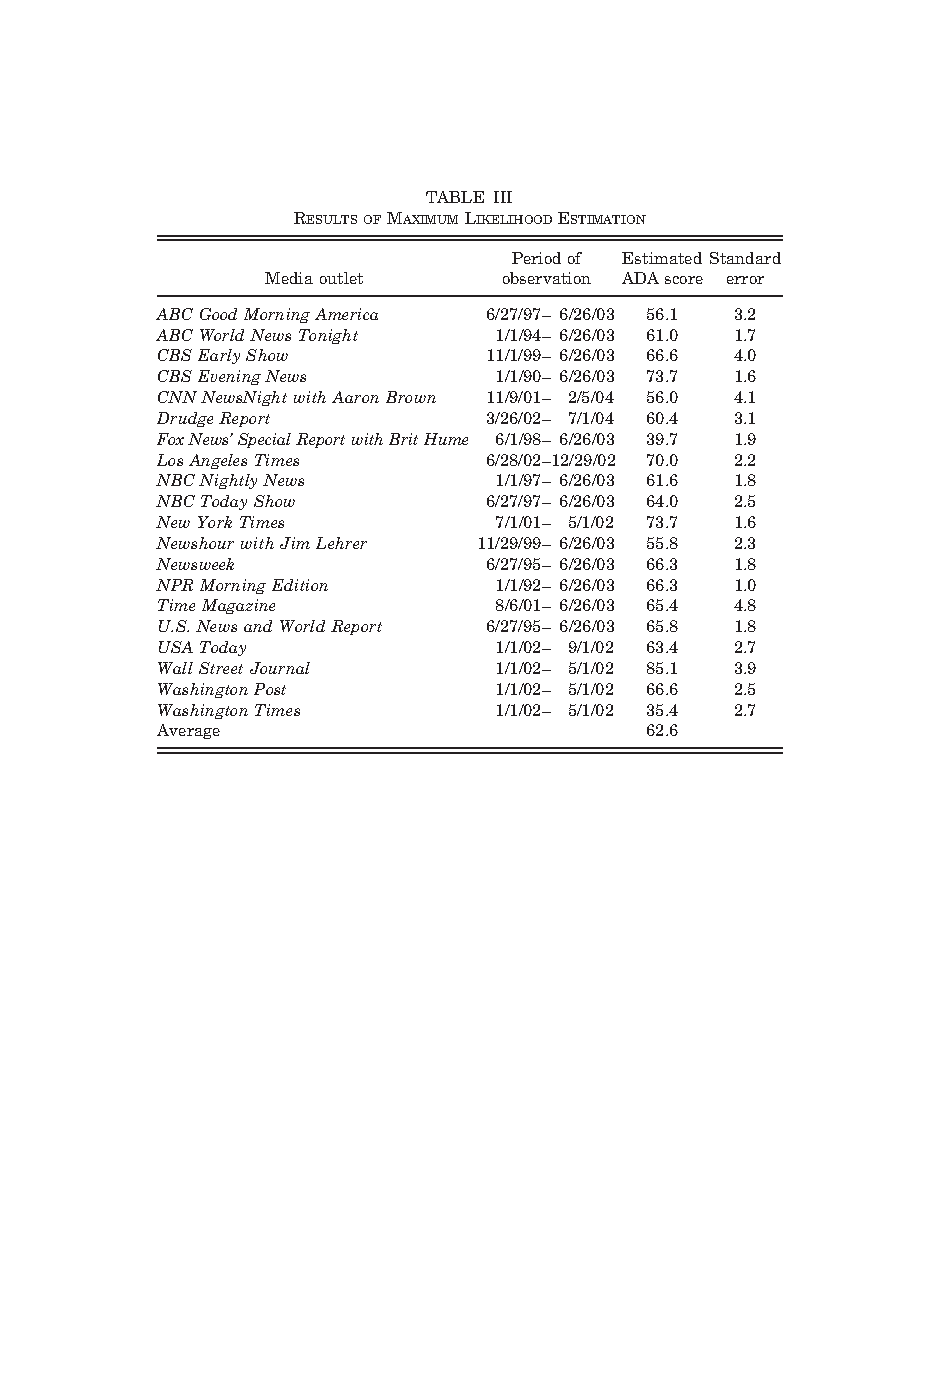
\includegraphics [width=0.9\vsize]{Images/groseclose_milyio_table1.pdf}
\end{center}
\end{figure}
\end{frame}

\begin{frame}
\frametitle{Results (cont.)}

\begin{figure}
\begin{center}
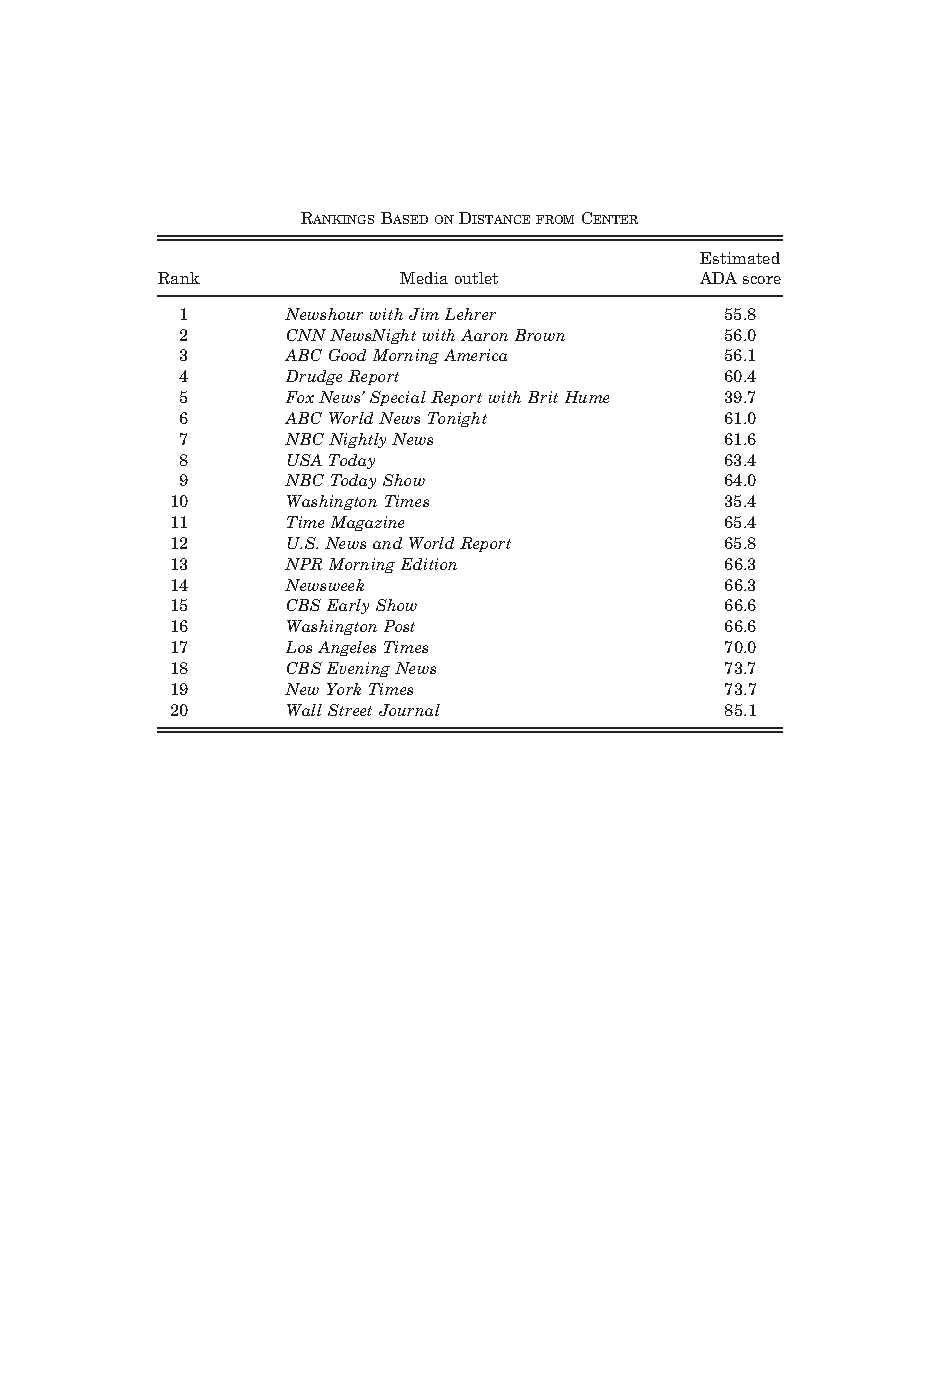
\includegraphics [width=0.9\vsize]{Images/groseclose_milyio_table2.pdf}
\end{center}
\end{figure}
\end{frame}

\begin{frame}
\frametitle{Results (cont.)}

\begin{figure}
\begin{center}
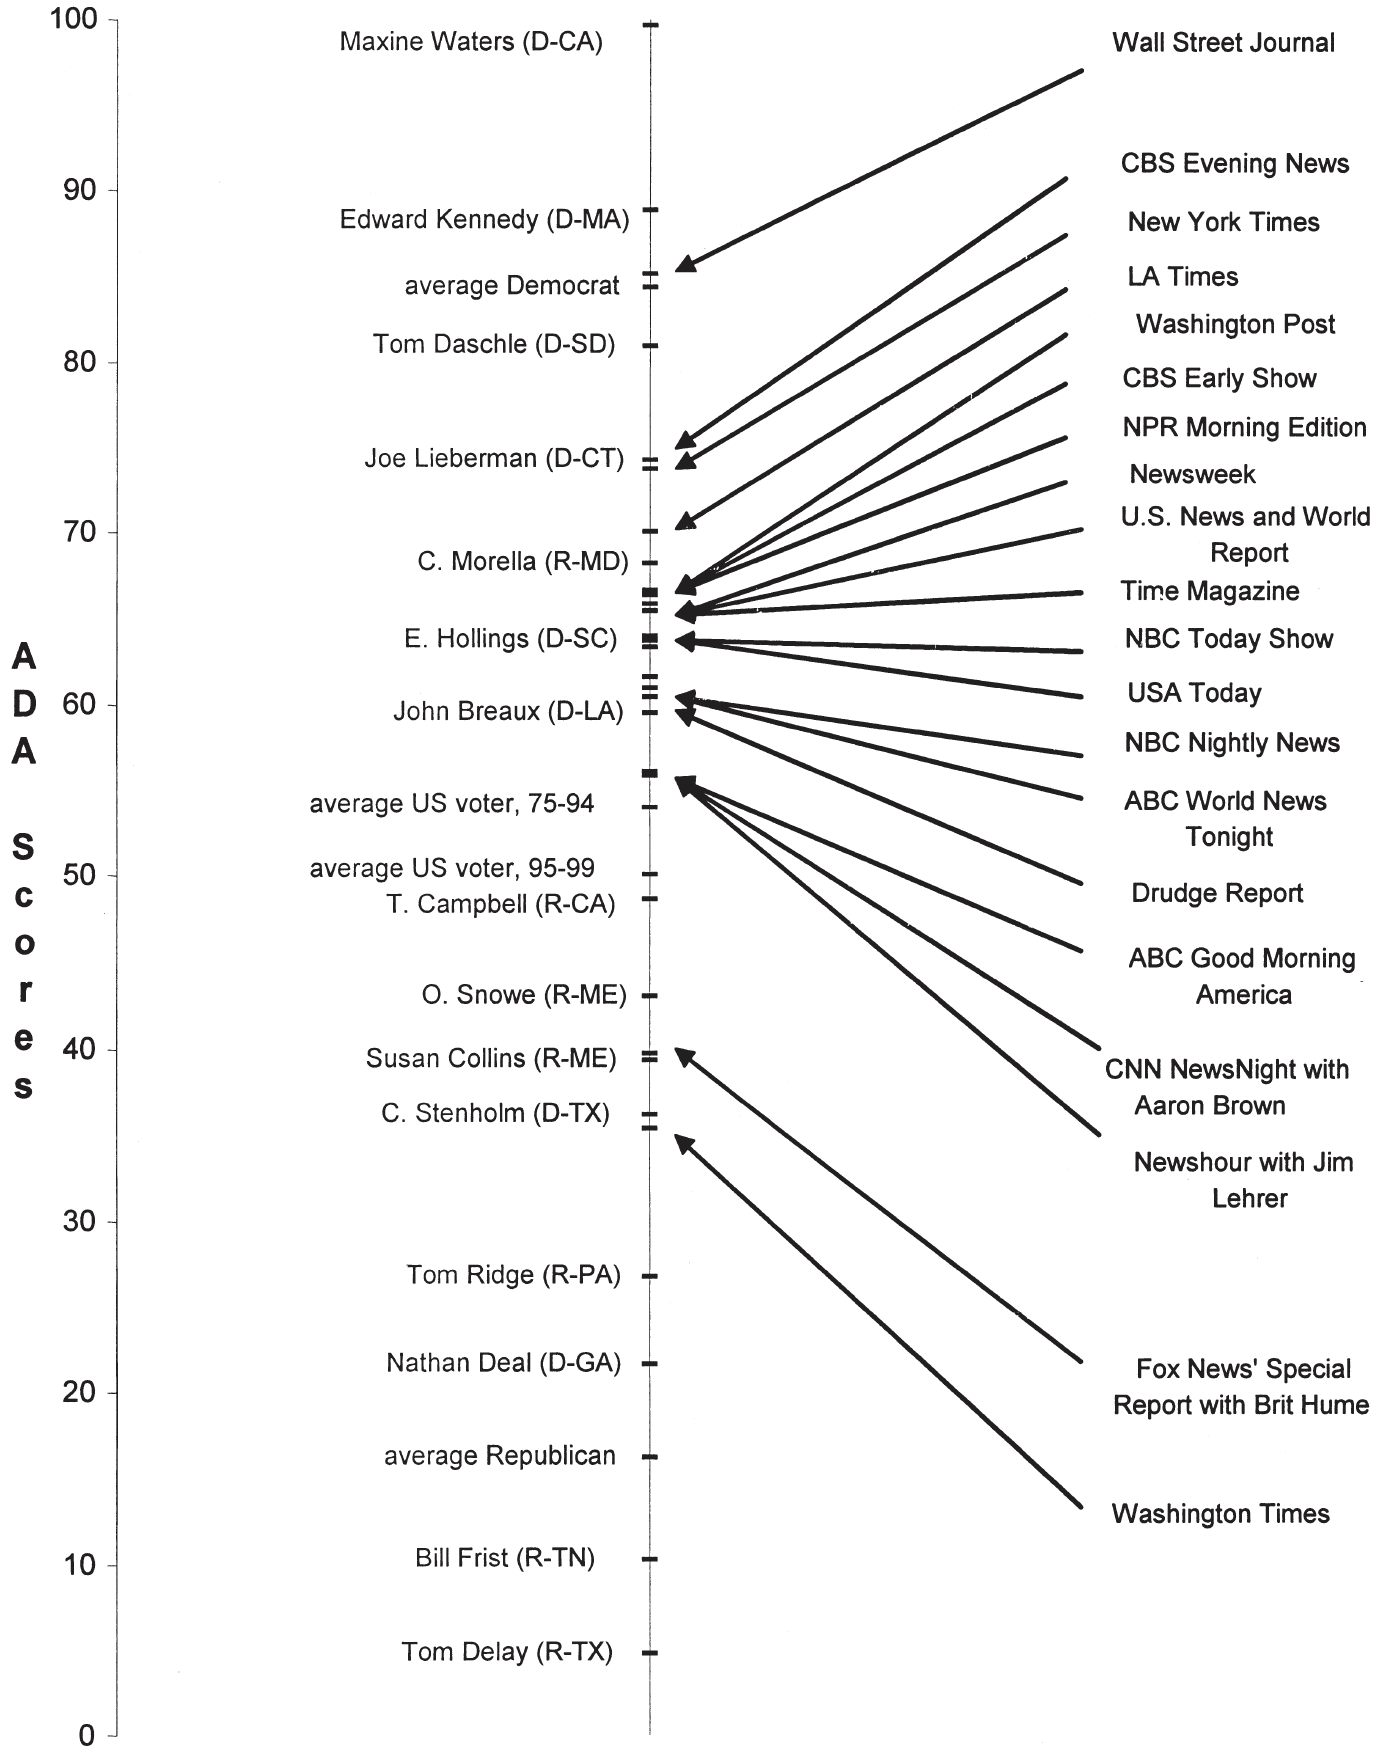
\includegraphics [width=0.7\vsize]{Images/groseclose_milyio_figure_2.png}
\end{center}
\end{figure}
\end{frame}

\begin{frame}{What Drives Media Slant (Gentzkow-Shapiro, 2010)}
\begin{itemize}
\setlength{\itemsep}{0.9em}

\item{\textcolor{blue}{\large Goal:}
\vspace*{5pt}
\begin{itemize}
\setlength{\itemsep}{0.5em}
\setlength{\itemindent}{-1em}
\item{Construct a measure of media slant based on the similarity of the \\
\hspace{-10pt}\textcolor{blue}{language} used by newspapers and politicians}
\end{itemize}}

\pause

\item{\textcolor{blue}{\large Methodology:}
\vspace*{5pt}
\begin{itemize}
\setlength{\itemsep}{0.5em}
\setlength{\itemindent}{-1em}
\item{Consider official speeches by US congressmen}
\item{Identify the two- and three-word expressions most representative of\\
\hspace{-10pt}\textit{Republicans} and \textit{Democrats}}
\item{Compute the frequency of ``Democratic'' and ``Republican'' \\
\hspace{-10pt}expressions in the articles published in over 400 newspapers}
\item Define the slant of each newspaper with respect to politicians
\item Test whether slant is driven by consumers' vs. owners' preferences
\end{itemize}}

\pause

\item{\textcolor{blue}{\large Findings:}
\vspace*{5pt}
\begin{itemize}
\setlength{\itemsep}{0.5em}
\setlength{\itemindent}{-1em}
\item{Slant highly correlated with political leaning of potential readers}
\item{Identity of media owner does not explain much} 
\end{itemize}}
\end{itemize}
\end{frame}


\begin{frame}{Data}
\begin{itemize}
\setlength{\itemsep}{1.2em}

\item{\textcolor{blue}{\large Politicians:}
\vspace*{5pt}
\begin{itemize}
\setlength{\itemsep}{0.5em}
\setlength{\itemindent}{-1em}
\item{All speeches from 2005 \textit{Congressional Record}}
\item{Ideological score: vote share to Bush in 2004 presidential election\\
\hspace{-10pt}in congressperson's constituency}
\end{itemize}}

\pause

\item{\textcolor{blue}{\large News content:}
\vspace*{5pt}
\begin{itemize}
\setlength{\itemsep}{0.5em}
\setlength{\itemindent}{-1em}
\item{Headlines and text of all articles published on 433 US daily\\
\hspace{-10pt}newspapers in 2005}
\item{Source: Newslibrary, ProQuest}
\item{Only news articles, no editorials}
\end{itemize}}

\pause

\item{\textcolor{blue}{\large Other:}
\vspace*{5pt}
\begin{itemize}
\setlength{\itemsep}{0.5em}
\setlength{\itemindent}{-1em}
\item{Newspaper HQ location and relevant market (PMSA)}
\item{Vote shares for Republicans and Democrats in relevant media market}
\item{Identity of newspaper's owner}
\end{itemize}}
\end{itemize}
\end{frame}

\begin{frame}
\frametitle{Methodology: step \#1}
\begin{itemize}
\setlength{\itemsep}{0.8em}

\item{Pre-process the \textit{Congressional Record} corpus: remove stop words, stemming (Porter)}
\pause
\item{Consider all 2-word and 3-word phrases appearing in the corpus}
\pause
\item{For each phrase $p$ of length $l$, compute the total number of times it is used by Democrats and Republicans (\textcolor{blue}{$f_{pld}, f_{plr}$})}
\pause
\item{For each phrase compute the Pearson's $\chi^{2}$ statistic: \\
$$ \chi_{pl}^2 = \frac{(f_{plr}f_{\sim pld} - f_{pld}f_{\sim plr})^2}{(f_{plr}+f_{pld})(f_{plr}+f_{\sim plr})(f_{pld}+f_{\sim pld})(f_{\sim plr}+f_{\sim pld})} $$
}

\pause
\item{$\chi^{2}$: test statistic for the null hypothesis that the propensity to use phrase $p$ is equal for Democrats and Republicans.}

\pause
\item{Simple to compute, only requires $f_{pld}$ and $f_{plr}$. Preferable to other naive statistics such as the ratio of uses by D or R}

\end{itemize}
\end{frame}

\begin{frame}
\frametitle{Methodology: step \#2}
\begin{itemize}
\setlength{\itemsep}{0.8em}

\item{Eliminate phrases that are not likely to be useful for diagnosing newspaper partisanship.}
\pause
\item{2-word phrases appearing less than 200 times in newspaper headlines (e.g., procedural phrases not used by the media)}
\item{2-word phrases that appeared more than 15,000 times in headlines (e.g., ``third quarter'' or ``exchange rate'')}
\item{3-word phrases that appeared less than 5 times in headlines}
\item{3-word phrases that appeared more than 1,000 times in headlines}
\item{Any phrase that appeared in the full text of more than 400,000 documents}
\pause
\item{Among the remaining ones, select the 500 phrases of each length with the highest values of $\chi_{pl}^2$}
\end{itemize}
\end{frame}

\begin{frame}
\frametitle{Most representative Democratic phrases}
\begin{center}
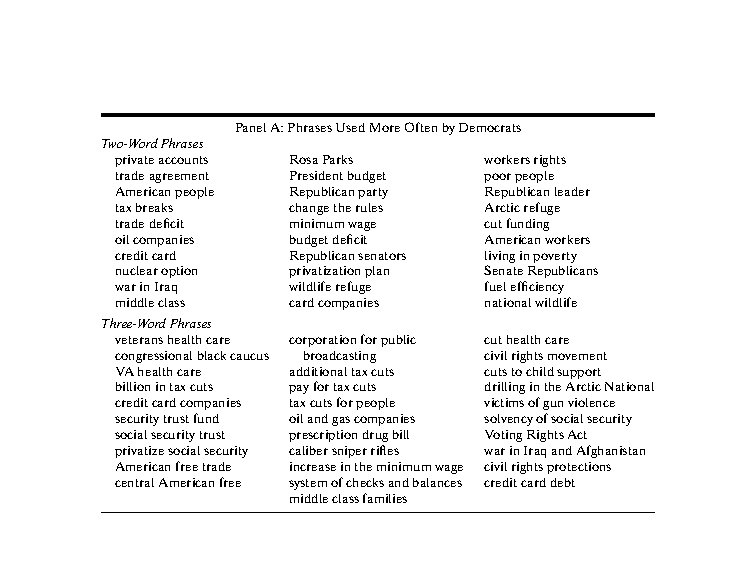
\includegraphics[scale=1.13]{Images/gentzkow_table1.pdf}
\end{center}
\end{frame}

\begin{frame}
\frametitle{Most representative Republican phrases}
\begin{center}
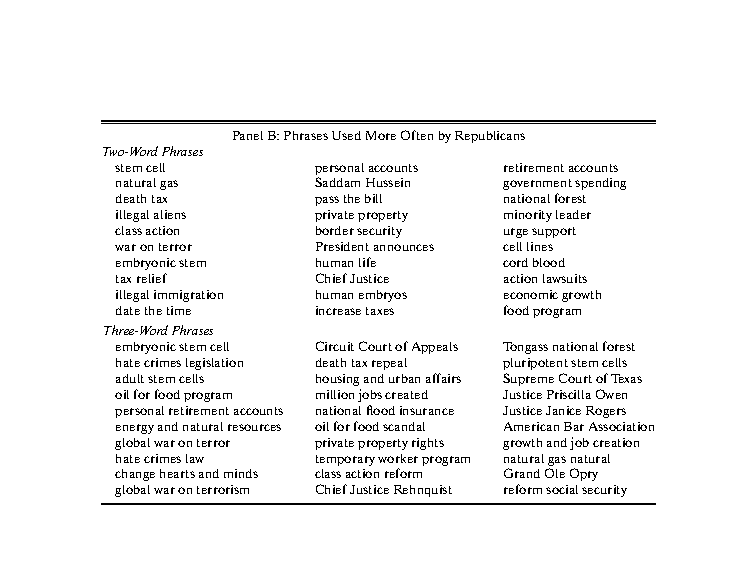
\includegraphics[scale=1.13]{Images/gentzkow_table2.pdf}
\end{center}
\end{frame}

\begin{frame}
\frametitle{Methodology: step \#3}
\begin{itemize}
\setlength{\itemsep}{0.8em}

\item{Use politicians' language and ideology to \textcolor{blue}{map phrases to ideology}}
\pause
\item{Re-index the phrases in the sample by \textcolor{blue}{$p \in [1,...,1000]$}}
\pause
\item{For each congressperson \textcolor{blue}{$c \in C$} we observe ideology \textcolor{blue}{$y_c$} and phrase frequencies \textcolor{blue}{$\{f_{pc}\}_{p=1}^{1000}$}}
\pause
\item{Compute relative frequencies as: \textcolor{blue}{$\tilde{f}_{pc}=f_{pc}/\sum{}_{p=1}^{P}f_{pc}$}}
\pause
\item{For each phrase \textcolor{blue}{$p$}, we regress \textcolor{blue}{$\tilde{f}_{pc}$} on \textcolor{blue}{$y_c$} for the sample of congresspeople, obtaining an intercept and a slope parameter, \textcolor{blue}{$a_p$} and  \textcolor{blue}{$b_p$}}
\pause
\item{Hence we estimate 1,000 separate regressions, each with a sample the size of \textcolor{blue}{$C$}}

\item{Intuition: the larger \textcolor{blue}{$b_p$} the more the use of a phrase is correlated with ideology (\textcolor{blue}{$y_c$})}
\end{itemize}
\end{frame}

\begin{frame}
\frametitle{Methodology: step \#4}
\begin{itemize}
\setlength{\itemsep}{0.8em}
\item{We want to assign each paper a measure of slant based on the frequency  of phrases it uses and their ideological valence}
\pause
\item{For each paper \textcolor{blue}{$n \in N$}, we observe the relative frequency for each phrase  \textcolor{blue}{$\tilde{f}_{pc}$}, but not the ideology  \textcolor{blue}{$y_n$}, which we want to estimate}
\pause
\item{For each newspaper  \textcolor{blue}{$n$} we regress \textcolor{blue}{$(\tilde{f}_{pn}-a_p)$} on \textcolor{blue}{$b_p$} for the sample of phrases, obtaining the slope estimate:
%\item{For each paper $n$, we regress $(\tilde{f}_{pc}− a_p)$ on $b_p$ for the sample of phrases, obtaining the slope estimate:}
%% 
$$ \hat{y}_n =  \frac{
\sum_{p=1}^{1000}b_p(\tilde{f}_{pn}-a_p) 
}{\sum_{p=1}^{1000}b_p^2}$$
}
\pause
\item{We estimate \textcolor{blue}{$N$} separate regressions, each with a sample of 1,000}
\pause
\item{Intuition: the higher the frequency (\textcolor{blue}{$\tilde{f}_{pn}$}) of more ideological phrases (\textcolor{blue}{$b_p$}), the higher the measure of slant (\textcolor{blue}{$\hat{y}_n$})}
\end{itemize}
\end{frame}

\begin{frame}{Validating the measure of slant}
\vspace{-7pt}
\begin{center}
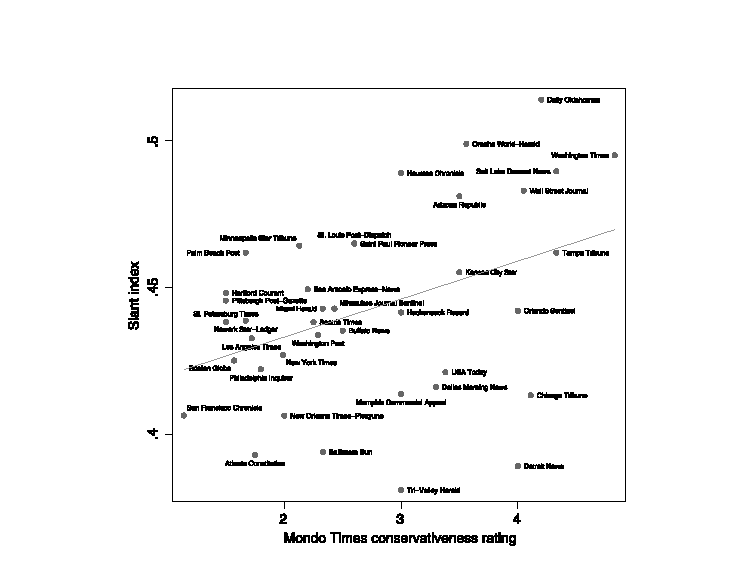
\includegraphics[scale=1]{Images/gentzkow_table3.pdf}
\end{center}
\end{frame}

\begin{frame}{Using the measure: slant and readers' ideology}
\vspace{-7pt}
\begin{center}
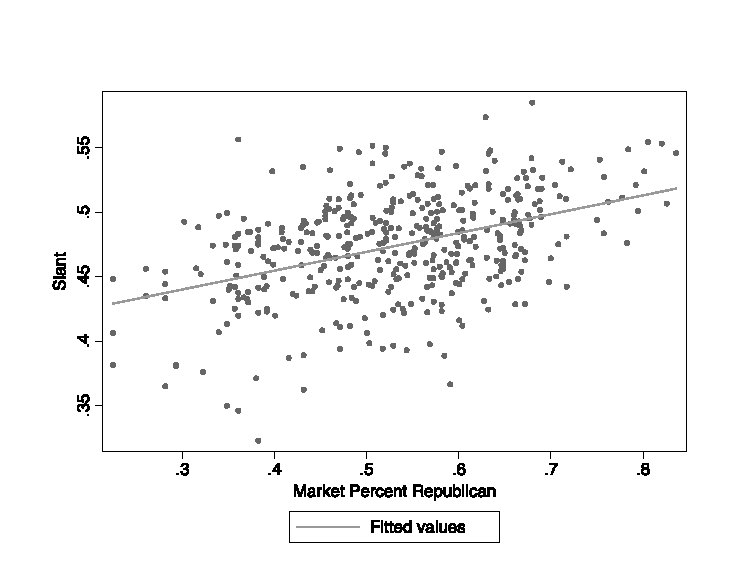
\includegraphics[scale=1]{Images/gentzkow_table4.pdf}
\end{center}
\end{frame}

\begin{frame}{Using the measure: slant and owners' ideology}
\vspace{-7pt}
\begin{center}
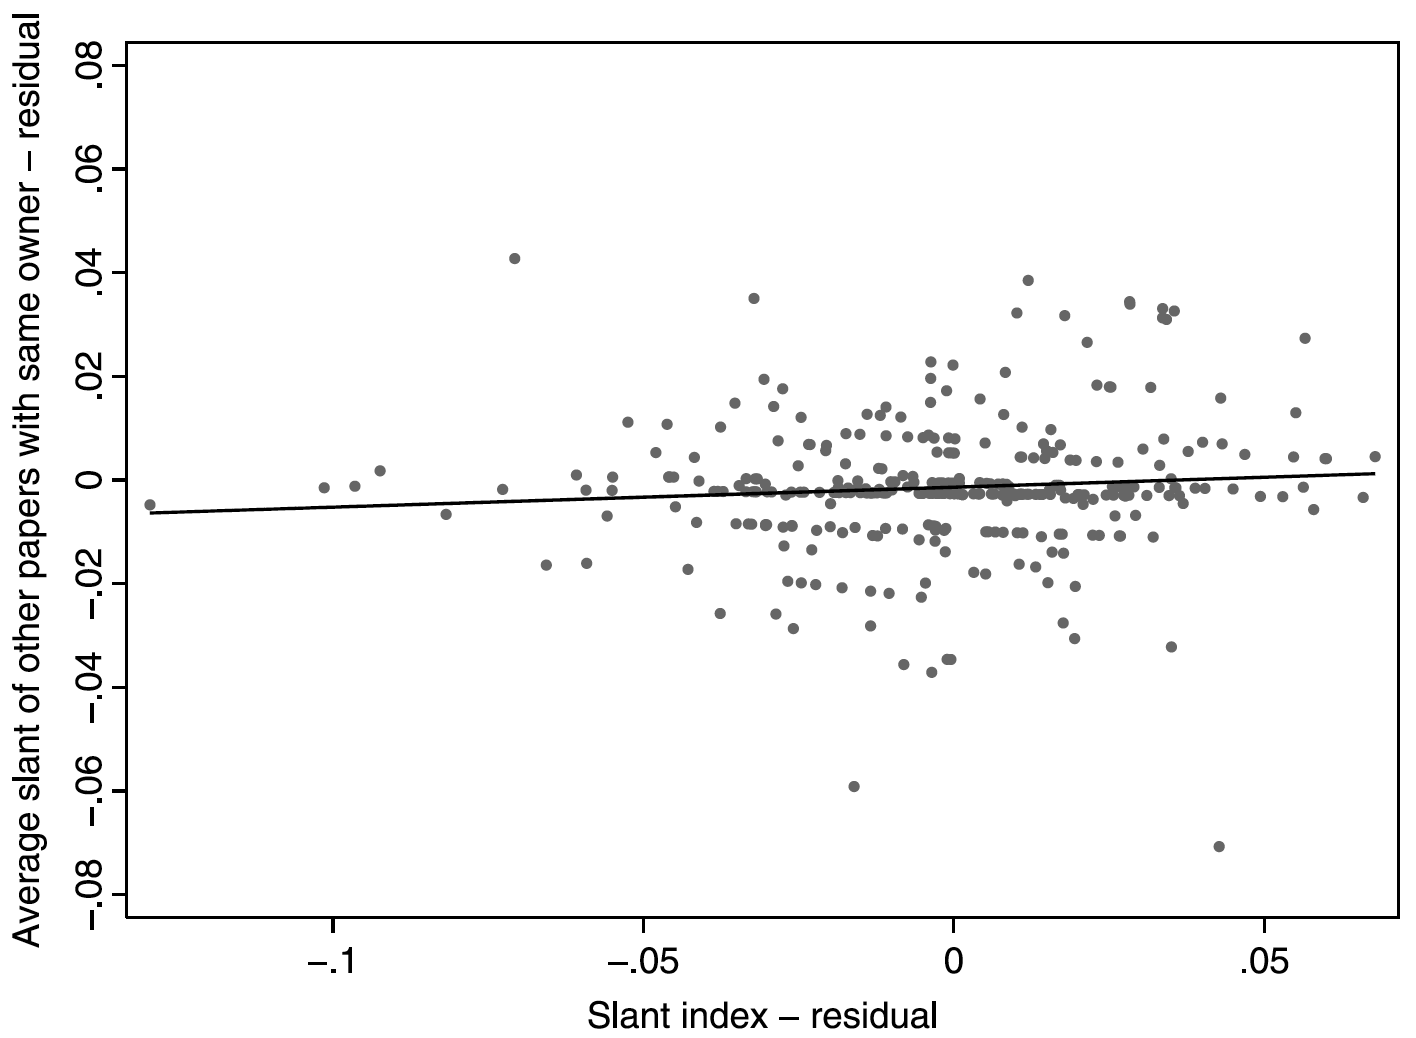
\includegraphics[scale=0.42]{Images/gentzkow_figure1}
\end{center}
\end{frame}

\begin{frame}{Using the measure: slant and owners' ideology}
\vspace{-7pt}
\begin{center}
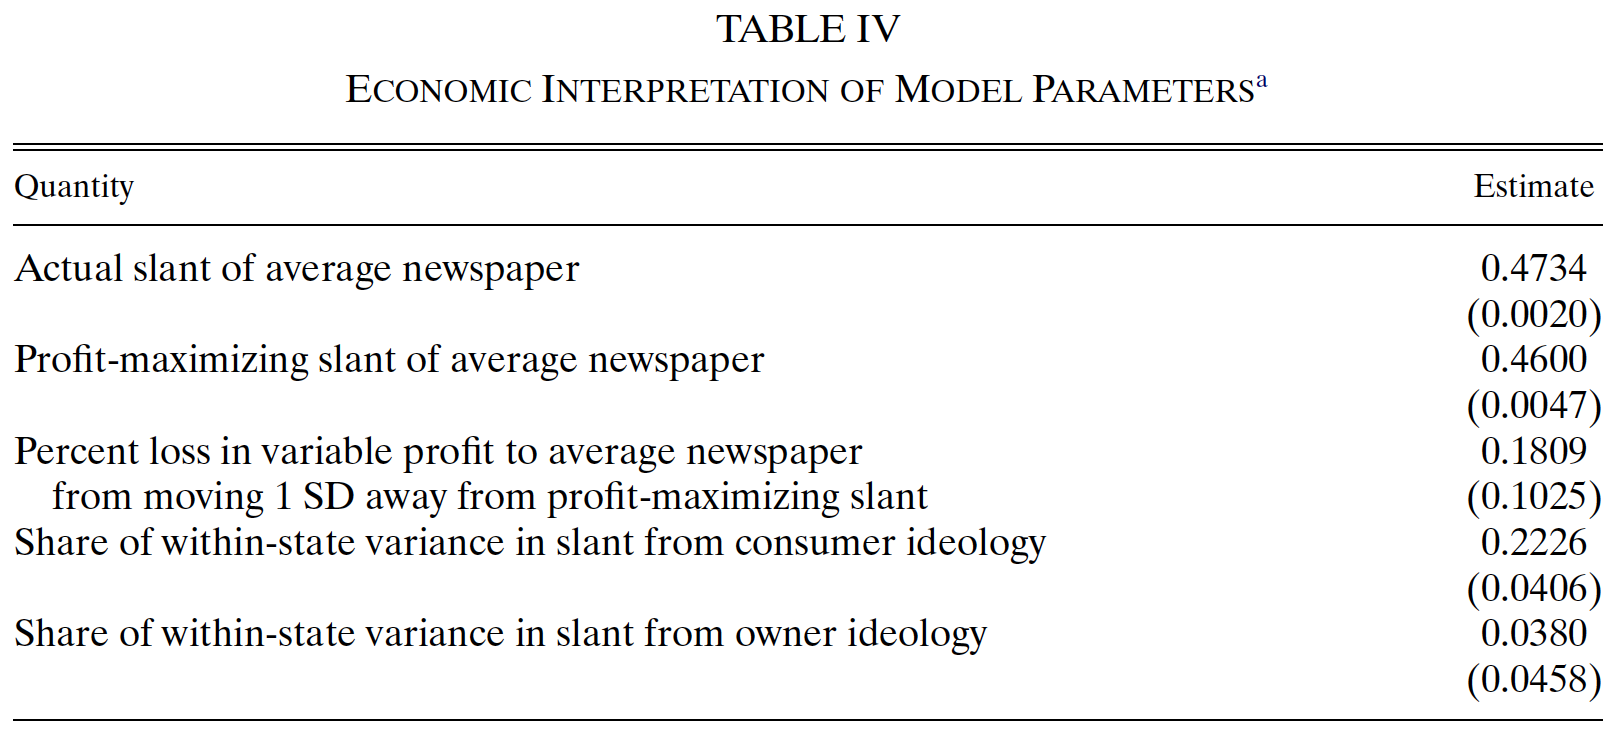
\includegraphics[scale=0.38]{Images/gentzkow_table5}
\end{center}
\end{frame}

\begin{frame}{Production of Information in an Online World \normalsize{(Cage et al., 19)}}
\begin{itemize}
\setlength{\itemsep}{1em}
    \item \textcolor{blue}{Goal:}
    \vspace*{5pt}
    \begin{itemize}
    \setlength{\itemsep}{0.4em}
        \item Study how much online media outlets \textcolor{blue}{copy content} from each other in the news production process
    \end{itemize}
    
    \pause
    
    \item \textcolor{blue}{Methodology}:
    \vspace*{5pt}
    \begin{itemize}
        \setlength{\itemsep}{0.4em}
        \item Consider all online news content produced by French media in 2013
        \item Identify 25K news events with an \textcolor{blue}{event-detection algorithm}
        \item Identify first news item that breaks news about an event
        \item Measure how much copying is used by subsequent news stories related to event with \textcolor{blue}{plagiarism detection algorithm}
        \item Measure effects of copying on readership/audience
    \end{itemize}
    
        \pause
        
    \item \textcolor{blue}{Findings:}
    \vspace*{5pt}
    \begin{itemize}
        \setlength{\itemsep}{0.4em}
        \item Online copying in news production is widespread: 61.8\% of content presents some form of copying
        \item Producing original content is rewarded with larger viewership shares
    \end{itemize}
    
\end{itemize}
\end{frame}


\begin{frame}{Data}
\begin{itemize}
    \setlength{\itemsep}{1.2em}
    \item \textcolor{blue}{Online News Content:}
    \vspace{4pt}
    \begin{itemize}
    \setlength{\itemsep}{0.6em}
        \item More than 2.5 million French news articles published online in 2013 (7K/day)
        \item \textcolor{blue}{Transmedia approach:}  content from 86 media outlets including 1 news agency (AFP), 59 newspapers, 10 online-only media outlets, 7 radio stations, 9 TV channels
        \item Source: French National Audiovisual Institute (public company)
    \end{itemize}
    
    \item  \textcolor{blue}{Viewership:}
   \vspace{4pt}
    \begin{itemize}
    \setlength{\itemsep}{0.4em}
        \item Daily audience measures for 58 out of the 86 outlets (AFP and some local newspapers not covered)
        \item Number of shares of the article on Facebook and Twitter. Proxy for the number of views of an article
        %Authors do a robustness exercise on articles published online by LeMonde for which they have real data on viewership at the article level for 5 months in 2017. Details on this later. They also use a media consumption survey with data in 2013 to see to what extent there is a selection bias of individuals sharing news on social media compared to ``regular viewers''. Analyses show that people who share news on social media are more likely to live in Ile De France and are younger. Selection comes mostly from age according to the authors.
    \end{itemize}
\end{itemize}
\end{frame}

\begin{frame}{Methodology: step \#1 event detection algorithm}
    \begin{itemize}
    \setlength{\itemsep}{0.8em}
        \item Consider headline and text of each article and compute its \textcolor{blue}{TF-IDF vector representation}
        \item Compute the cosine similarity of each article-pair
        \item Iteratively aggregate articles into \textcolor{blue}{event-clusters} if the cosine similarity is above a certain threshold (determined manually)
        \item ``Close'' an event if no article is aggregated to it within a 24-hour window
        \item Drop events that contain less than 2 distinct media outlets and less than 10 articles.
        \item Results in \textcolor{blue}{25,215 news events}, each lasting about 41 hours
        \item 33.4\% of of the 2.5M articles are classified into an event %The others are not used in the analysis (mostly local news stories, one-off reports or opinion pieces).
        \item Very large clusters are mostly \textcolor{blue}{``garbage clusters''}
    \end{itemize}
\end{frame}

\begin{frame}{Methodology: step \#2 plagiarism detection algorithm}
    \begin{itemize}
\setlength{\itemsep}{0.8em}
 \item Consider all the articles within an event-cluster and order them by time. The first one is the \textcolor{blue}{news-breaking article}.
\item Define the \textcolor{blue}{reaction time} of an article as the time elapsed since publication of the news-breaking article
\item Compare the text of each article to that of all the preceding articles in the event-cluster
\item If a portion of text of at least 100 characters in the article is identical to any previous portion that is already published, then that portion is defined as a \textcolor{blue}{copy}
        \item For each article, calculate the \textcolor{blue}{originality rate}, defined as:
        \begin{equation*}
            \text{originality rate } = \frac{\text{\# original characters}}{\text{\# total characters}}
        \end{equation*}
    \end{itemize}
\end{frame}


\begin{frame}{Summary statistics}
\begin{center}
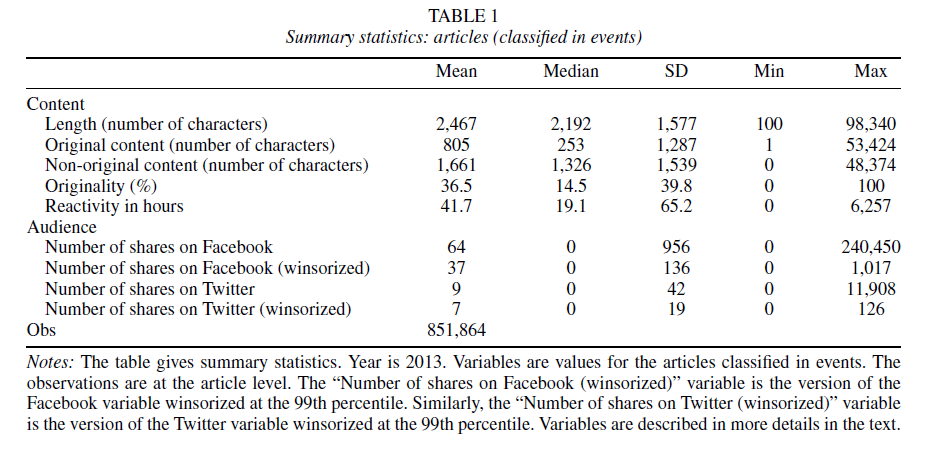
\includegraphics[width=1.05\textwidth]{Images/cage-1.PNG}
\end{center}
\end{frame}
%

\begin{frame}{Originality rate distribution}
    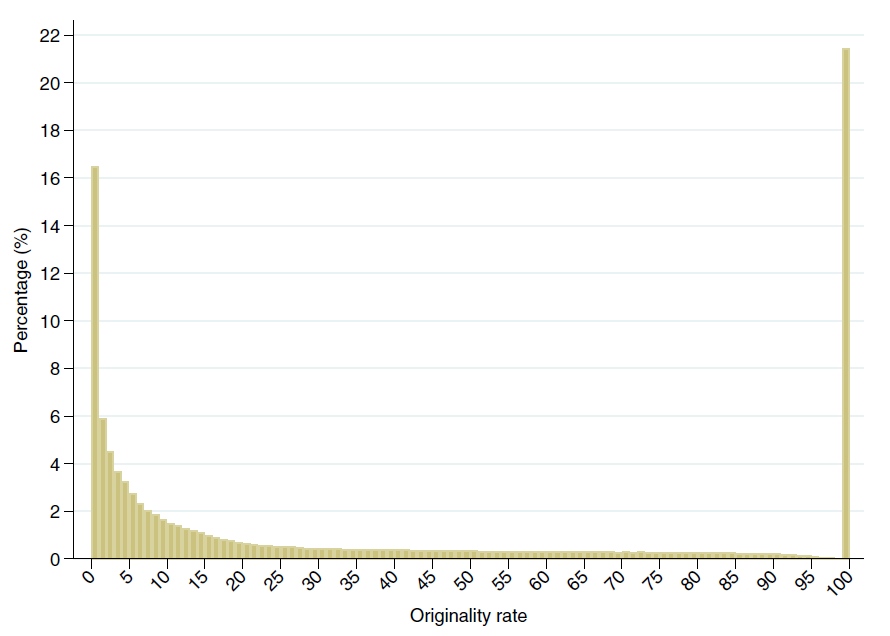
\includegraphics[width=1\textwidth]{Images/cage-5.PNG}
\end{frame}
%

\begin{frame}{Positive relationship between originality and reaction time}
    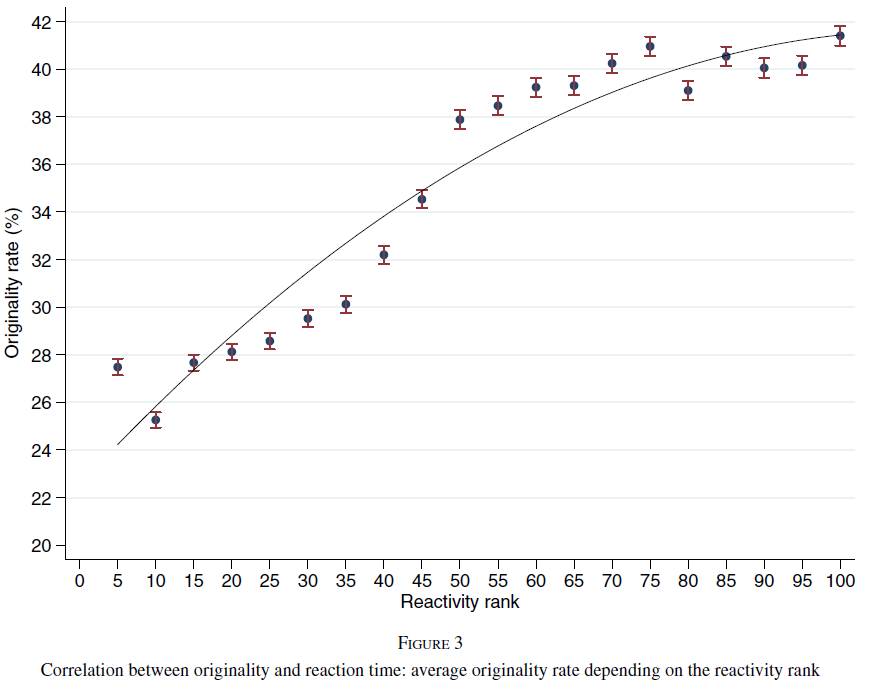
\includegraphics[width=1\textwidth]{Images/cage-2.PNG}
\end{frame}

\begin{frame}{Methodology: step \#3 strategies to proxy article views}
    \begin{itemize}
    \setlength{\itemsep}{0.8em}
        \item \textcolor{blue}{``Naive'' approach:}
        \begin{itemize}
        \setlength{\itemsep}{0.3em}
            \item On a given day and for a given outlet, assume all articles are equally popular
            \item Number of views is naively defined as number of page views on website divided by number of articles
        \end{itemize}
        \pause
        \item \textcolor{blue}{Linear approach:}
        \begin{itemize}
        \setlength{\itemsep}{0.3em}
            \item Number of article views is proportional to the relative number of shares of the article, within its outlet-day pair
        \end{itemize}
                \pause
        \item \textcolor{blue}{Social media approach:}
        \begin{itemize}
        \setlength{\itemsep}{0.3em}
            \item Collect data from leading French newspaper \textit{Le Monde} on \textcolor{blue}{article views} from April to August 2017
        \item Link the URL of the online article to Facebook (resp. Twitter) data in order to identify the number of shares on social media
        \item Examine correlation between the number of views on \textit{Le Monde} website and the number of social media shares
        \item Use relationship to infer the number of views for other outlets
        \end{itemize}
    \end{itemize}
\end{frame}


\begin{frame}{Social media shares and actual online views}
\begin{center}
 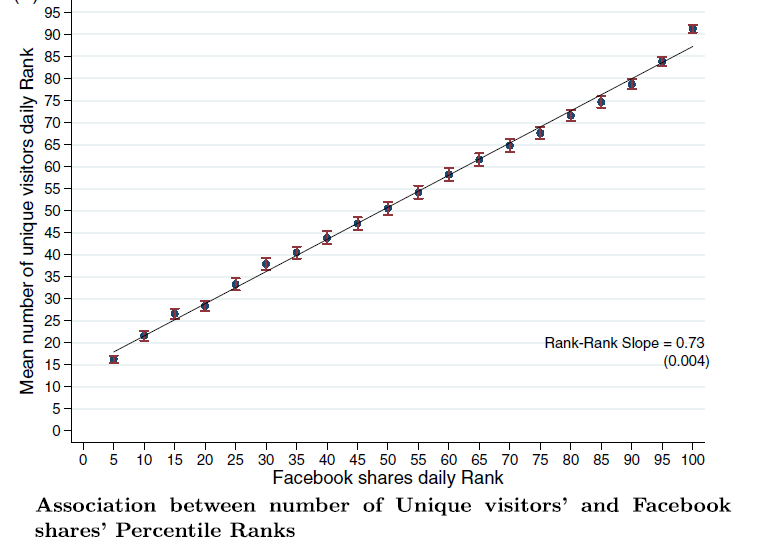
\includegraphics[width=1\textwidth]{Images/cage-6.PNG}
\end{center}
\end{frame}


\begin{frame}{Positive relationship between popularity and originality}
    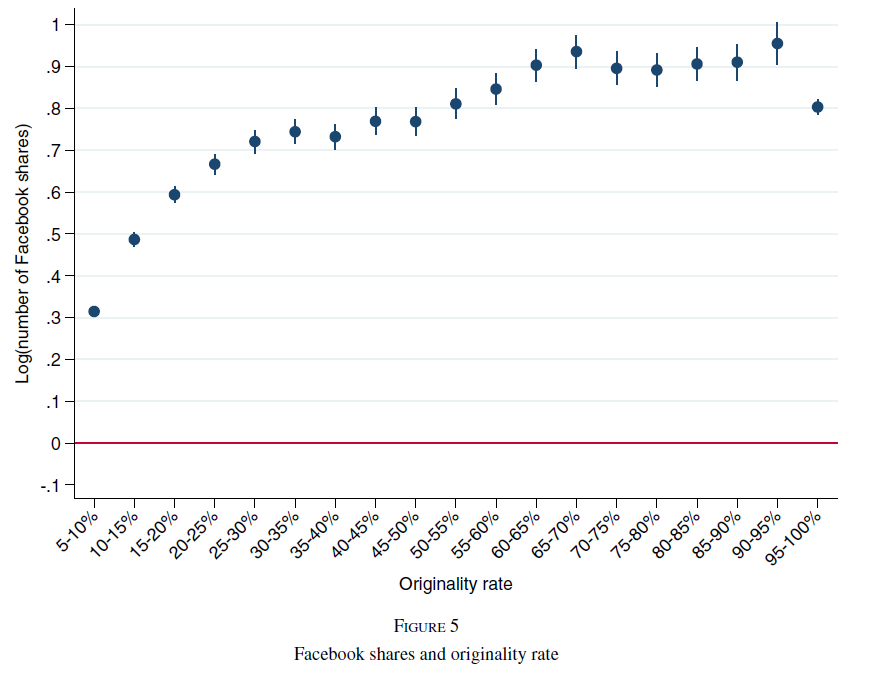
\includegraphics[width=1\textwidth]{Images/cage-3.PNG}
\end{frame}


\begin{frame}{Share of original content in articles data}
    \setlength{\itemsep}{0.8em}
        \tiny
        \begin{equation*}
            \frac{\sum_a \text{original content}_a \cdot \text{number of views}_a}{\sum_a \text{original content}_a \cdot \text{number of views}_a + \sum_a \text{non-original content}_a \cdot \text{number of views}_a}
        \end{equation*}
    
\begin{figure}
    \centering
    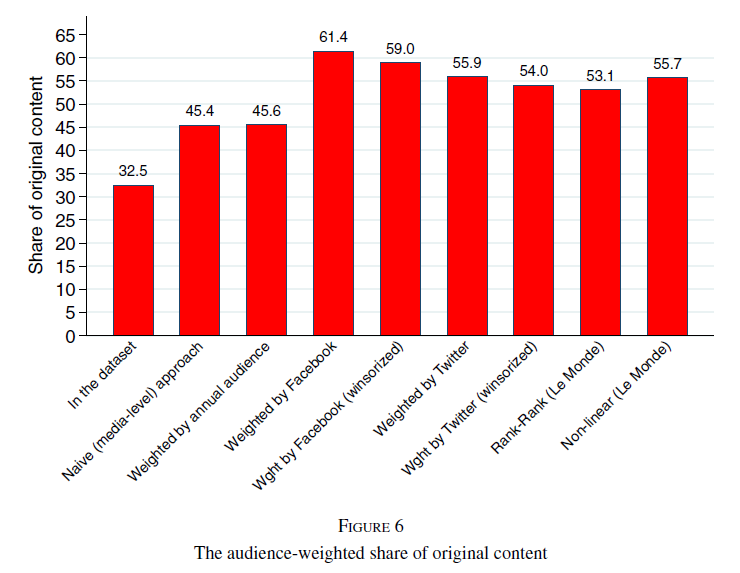
\includegraphics[scale = 0.65]{Images/cage-4.PNG}
\end{figure}
\end{frame}


\end{document}

